%%%%%%%%%%%%%%%%%%%%%%% file template.tex %%%%%%%%%%%%%%%%%%%%%%%%%
%
% This is a general template file for the LaTeX package SVJour3
% for Springer journals.          Springer Heidelberg 2010/09/16
%
% Copy it to a new file with a new name and use it as the basis
% for your article. Delete % signs as needed.
%
% This template includes a few options for different layouts and
% content for various journals. Please consult a previous issue of
% your journal as needed.
%
%%%%%%%%%%%%%%%%%%%%%%%%%%%%%%%%%%%%%%%%%%%%%%%%%%%%%%%%%%%%%%%%%%%

\documentclass[smallextended]{svjour3}       % onecolumn (second format)
\smartqed  % flush right qed marks, e.g. at end of proof
\usepackage{natbib}
\usepackage{tikz}
\usepackage{graphicx}
\usepackage{multirow}
\usepackage{amsmath}
\usepackage{amsfonts}
\usepackage{bigstrut}
\usepackage{color}
\usepackage{float}
\usepackage{graphics}
\usepackage{colortbl}
\usepackage[scaled=1]{helvet} 
\usepackage{balance}
\usepackage[shortlabels]{enumitem}
\usepackage{url}
\usepackage{rotating}
\usepackage[framed]{ntheorem}
\usepackage{framed}
\usepackage{hyperref}
\usepackage{subfig}

%% Caption font size
\usepackage[font=small]{caption}

%%% Color Definitions
\definecolor{lightgray}{gray}{0.8}
\definecolor{darkgray}{gray}{0.5}
\definecolor{lightgreen}{rgb}{.68, .79, .46}
\definecolor{lavenderpink}{gray}{0.92}
\definecolor{celadon}{gray}{0.7}
\definecolor{Gray}{gray}{0.9}
\definecolor{LightGray}{gray}{0.975}
\definecolor{cellgrey}{rgb}{.87, .87, .87}
\definecolor{steel}{rgb}{.11, .11, .7}
\definecolor{shadecolor}{gray}{0.95}


%%% Result Box
\newcommand{\result}[1]{
\vspace{0.2cm}
\noindent\begin{minipage}{\linewidth}
\begin{tabular}{|p{0.95\linewidth}|}
\hline\vspace{-0.2cm}
\textbf{\textit{\underline{Result}:}}~#1\\\hline
\end{tabular}
\end{minipage}\bigstrut
}

%%% Some shorthands
\newcommand{\bi}{\begin{itemize}} %[leftmargin=0.4cm]}
\newcommand{\ei}{\end{itemize}}
\newcommand{\be}{\begin{enumerate}}
\newcommand{\ee}{\end{enumerate}}
\newcommand{\ktest}{$\mathbb{K}$-test}
\newcommand{\tion}[1]{\S~\ref{sect:#1}}
\newcommand{\fig}[1]{Fig.~\ref{fig:#1}}
\newcommand{\tab}[1]{Table ~\ref{tab:#1}}
\newcommand{\eq}[1]{Equation~\ref{eq:#1}}
\newcommand{\review}[1]{\noindent\textit{#1\\}}


%%%%%%%%%%%%%%%%%%%%%%%%%%%%%%%%%%%%%%%%%%%%%%%%%%%%%%%%%%%%%%%%%%%%%%%%%%%%%%%%%%%%%%%%%%%%%%%%%%%%%%%%%%%%%%%%%%%%%%%%%%%%%%%%%%%%%%%%%%%%%%%%%%%%%%%%%%%%%%

%% BEGIN DOCUMENT

%%%%%%%%%%%%%%%%%%%%%%%%%%%%%%%%%%%%%%%%%%%%%%%%%%%%%%%%%%%%%%%%%%%%%%%%%%%%%%%%%%%%%%%%%%%%%%%%%%%%%%%%%%%%%%%%%%%%%%%%%%%%%%%%%%%%%%%%%%%%%%%%%%%%%%%%%%%%%%
\begin{document}

\title{Learning Actionable Analytics from Across Software Projects}

%\titlerunning{Short form of title}        % if too long for running head

\author{Rahul Krishna         \and
        Tim Menzies %etc.
}

%\authorrunning{Short form of author list} % if too long for running head

\institute{Rahul Krishna \at
          Computer Science \\
          NC State University \\
          \email{i.m.ralk@gmail.com}           %  \\
           \and
           Tim Menzies \at
          Computer Science \\
          NC State University \\
          \email{timm@ieee.org}           %  \\
}

\date{Received: date / Accepted: date}
% The correct dates will be entered by the editor


\maketitle

\begin{abstract}
The current generation of software analytics tools are mostly prediction algorithms (e.g. support vector machines, naive
bayes, logistic regression, etc). While prediction is useful, after prediction comes planning about what actions to take in order to
improve quality. This research seeks methods that generate demonstrably useful guidance on “what to do” within the context of a
specific software project. Specifically, we propose XTREE (for within-project planning) and BELLTREE (for cross-project planning) to
generating plans that can improve software quality. Each such plan has the property that, if followed, it reduces the probability of future
defect reports. When compared to other planning algorithms from the SE literature, we find that this new approach is most effective at
learning plans from one project, then applying those plans to another. In 10 open-source JAVA systems, several hundreds of defects
were reduced in sections of the code that followed the plans generated by our planners. Further, we show that planning is possible
across projects, which is particularly useful when there are no historical logs available for a particular project to generate plans from.
\keywords{Data Mining, Actionable Analytics, Planning, bellwethers, defect prediction.}
% \PACS{PACS code1 \and PACS code2 \and more}
% \subclass{MSC code1 \and MSC code2 \and more}
\end{abstract}

\section{Introduction}
Data mining tools have been applied to many applications in SE (e.g.~\cite{czer11, ostrand04, Menzies2007a, turhan11, koc11b, export:208800, theisen15}). 
Despite these successes,  current
software analytic tools have certain drawbacks. At a workshop on ``Actionable Analytics'' at the 2015 IEEE conference on
Automated Software Engineering, 
business users were vocal in their complaints about analytics~\cite{hihn15}.
``Those tools tell us \textit{what is}, '' said one business user, ``But they don't tell us \textit{what to do}''.
Hence we seek new tools that offer  guidance on ``what to do'' within a specific project. 

We seek such new tools since  current   analytics tools are mostly \textit{prediction} algorithms such as support vector machines~\cite{cortes95}, naive Bayes classifiers~\cite{lessmann08}, logistic regression~\cite{lessmann08}. For example, defect prediction tools report what combinations of software project features predict for some dependent variable (such as the number of defects). Note that this is a different task to \textit{planning}, which answers the question: what to {\em change} in order to {\em improve} quality.
	
More specifically, we seek plans that offer {\em least} changes in software but most \textit{improve} the \textit{quality}; here:
\bi
\item \textit{Quality} = defects reported by the development team; 
\item \textit{Improvement} = lowered likelihood of future defects.
\ei
This paper advocates the use of the {\em bellwether effect}~\cite{krishna16, krishna17a, mensah2018investigating} to generate plans. This effect states that:
\begin{quote}
  \textit{`` \ldots When a community of programmers work on a set of projects, then within that community there exists one exemplary project, called the bellwether\footnote{According to the Oxford English Dictionary, the bellwether is the leading sheep of a flock, with a bell on its neck.}, which can best define quality predictors for the other projects \ldots ''}
\end{quote}
Utilizing the bellwether effect, we propose a cross-project variant of our XTREE contrast set learner called BELLTREE (a portmanteau,  \textit{BELLTREE} = \textit{Bellwether}$+$\textit{XTREE}). 

BELLTREE searches for an exemplar project, or \textit{bellwether}~\cite{krishna17a}, to construct plans from other projects. As shown by
the experiments of this paper, these plans can be remarkably effective. In 10 open-source JAVA systems, hundreds of defects could potentially be reduced in sections of the code that followed the plans generated by our planners. Further, we show that planning is possible across projects, which is particularly useful when there are no historical logs available for a particular project to generate plans from.


The structure of this paper is as follows: the rest of this section introduces the four research questions asked in this paper, our contributions (\tion{contrib}), and relationships between this and our prior work (\tion{our_prior}). In \tion{motivate} we discuss the notion of planning. There, in \tion{planners}, we discuss the planners studied here. \tion{prelim} contains the research methods, datasets, and evaluation strategy. In \tion{results} we answer the research questions. In \tion{discuss} we discuss the implications of our findings. Finally, \tion{threats} and \tion{future} present threats to validity and conclusions respectively.

\subsubsection*{RQ1: Is within-project planning with XTREE comparatively more effective?}

In this research question, we explore what happens when XTREE  is trained on past data from \textit{within} a project. XTREE uses
historical logs from past releases of a project to recommend changes that might reduce defects in the next version of the software. Since such effects might not actually be casual, 
our first research question compares 
the effectiveness of XTREE's recommendations against  alternative planning methods. Recent work by Shatnawi~\cite{shatnawi}, Alves et al.~\cite{alves}, and Oliveira et al.~\cite{oliveira} assume that unusually large measurements in source code metrics point to larger likelihood of defects. Those
planners recommend changing all such unusual code since they assume that, otherwise, this may lead to defect-prone code. When XTREE is compared to the methods
of Shatnawi, Alves, Oliveira et al., we find that: 

\result{Planning with XTREE leads to the largest number of defects being reduced. This was true in 9 out of 10 projects studied here. Also, plans generated by XTREE are superior to other methods in all 10 projects.}

\vspace{2mm}
\noindent Here, by ``superior'' we mean ``larger defect reduction''.

\subsubsection*{RQ2: Is cross-project planning with BELLTREE effective?}
  
This research question addresses cases where projects lack local data (perhaps due to the project being relatively new). We ask if we can move data {\em across}
from other projects to generate actionable plans.

For prediction tasks, in the case of domains like defect prediction, effort estimation, code smell detection, etc., it has been shown that the \textit{bellwether effect}~\cite{krishna17a} can be used to make cross-project prediction when a project lacks sufficient within-project data. We ask if a similar approach is possible for planning across projects. To assert this, we first discover a \textit{bellwether} dataset from the available projects, and then we construct the BELLTREE planner. 

As with RQ1, we note that in a cross-project setting, plans generated using BELLTREE were  effective in generating actionable plans. Also, when compared plans from
Shatnawi, Alves, Oliveira et al., we find BELLTREE to be a significantly superior approach to cross-project planning.

\result{For cross-project planning, we see that recommendations from BELLTREE produces large reductions in the number of defects. This was true in 8 out of 9 projects studied here. Further, plans generated by BELLTREE were significantly superior to other planners.}


\subsubsection*{RQ3: Are cross-project plans generated by BELLTREE as effective as within-project plans of XTREE?}

In this research question, we compare the effectiveness of plans obtained with BELLTREE (cross-project) to plans obtained with XTREE (within-project). 

This is an important result---when local data is missing,  projects can use lessons learned from other projects.

\result{The effectiveness of BELLTREE is comparable to the effectiveness of XTREE.}

\subsubsection*{RQ4: How many changes do the planners propose?}

In the final research question, we ask how many attributes are recommended to be changed by different planners.

This result has a lot of practical significance since developers have a hard time following those plans that recommend too many changes.


\result{XTREE/BELLTREE recommends the least number of changes compared to other planners,  while also producing the best overall performance (measured in
terms of defect reduction).}

\subsection{Contributions}
\label{sect:contrib}
\textit{1. New kinds of software analytics techniques:} This work combines planning~\cite{krishna17a} with cross-project learning using bellwethers~\cite{krishna16}. This is a unique approach since our previous work on bellwethers~\cite{krishna16, krishna17b} explored prediction and not planning as described here. Also, our previous work on planning~\cite{krishna17a} explored with-project problems but not cross-project problems as explored here. 

\textit{2. Compelling results about planning:} Our results show that planning is quite successful in producing actions that can reduce the number of defects; Further, we see that plans learned on one project can be translated to other projects.

\textit{3. More evidence of generality of bellwethers:}  Bellwethers were
originally just used in the context of prediction~\cite{krishna16} and have been shown to work for (i)~defect prediction, (ii)~effort estimation, (iii)~issues close time, and (iv)~detecting code smells~\cite{krishna17b}. This paper extends those results with a new finding that bellwethers can also be used from cross-project planning. This is an important result of much significance since, it suggests that general conclusions about SE can be easily found (with bellwethers).

\textit{4. An open source reproduction package containing all our scripts and data.} For readers interested in replicating this work, kindly see \url{https://git.io/fNcYY}.
 
 
\begin{figure}[!b]
\centering
\resizebox{\linewidth}{!}{
\begin{tabular}{clcccl}
\multicolumn{1}{l}{}                       &                                                  & \multicolumn{3}{c}{Data source}                                                                                                       &  \bigstrut\\ \cline{3-5}
\multicolumn{1}{l}{}                       & \multicolumn{1}{l|}{}                            & \multicolumn{1}{c|}{Within}                   & \multicolumn{2}{c|}{Cross}                                                     &  \bigstrut\\ \cline{1-5}
\multicolumn{1}{|c|}{\multirow{5}{*}{Task}} & \multicolumn{1}{l|}{\multirow{3}{*}{Prediction}} & \multicolumn{1}{c|}{\multirow{3}{*}{TSE '07~\cite{menzies07}}} & \multicolumn{1}{l|}{EMSE '09~\cite{turhan09}}  & \multicolumn{1}{c|}{\multirow{3}{*}{TSE '17~\cite{fu18}}} &  \bigstrut\\
\multicolumn{1}{|c|}{}                      & \multicolumn{1}{l|}{}                            & \multicolumn{1}{c|}{}                         & \multicolumn{1}{l|}{ASE '16~\cite{krishna16}}   & \multicolumn{1}{c|}{}                         &  \bigstrut\\
\multicolumn{1}{|c|}{}                      & \multicolumn{1}{l|}{}                            & \multicolumn{1}{c|}{}                         & \multicolumn{1}{l|}{TSE '18~\cite{krishna17b}}   & \multicolumn{1}{c|}{}                         &  \bigstrut\\ \cline{2-5}
\multicolumn{1}{|c|}{}                      & \multicolumn{1}{l|}{Planning}                    & \multicolumn{1}{c|}{IST '17~\cite{krishna17a}}                  &  { \cellcolor{lightgray}This work}    &
\multicolumn{1}{l|}{Future work} &  \bigstrut\\ \cline{1-5}
\multicolumn{1}{l}{}                       & \multicolumn{1}{l|}{}                            & \multicolumn{2}{c|}{Homogeneous}                                               & \multicolumn{1}{c|}{Heterogeneous}            &  \bigstrut\\ \cline{3-5}
\end{tabular}}
 \caption{Relationship of this paper to our prior research. 
%Within project trained and tested data miners using data from the same project. Cross projects train on one project, then test on another. Homogeneous learning requires the attribute names to be identical in the training and test set. Heterogeneous learning relaxes that requirement; i.e. the attribute names might change from the training to the test set.
}
\label{fig:analytics}
 \end{figure}


\subsection{Relationship to Prior Work}
\label{sect:our_prior}
As for the connections to prior research, this article significantly extends those results.
As shown in \fig{analytics}, originally in 2007 we explored software quality prediction in the context of training and testing within the same software project~\cite{menzies07}. After that we found ways in 2009 to train these predictors on some projects, then test them on others~\cite{turhan09}. Subsequent work in 2016 found that bellwethers were a simpler and effective way to implement transfer learning~\cite{krishna16}, which worked well for a wide range of software analytics tasks~\cite{krishna17b}. Meanwhile, in the area of planning, we conducted some limited within-project planning in 2017 on recommending what to change in software~\cite{krishna17a}. This current article now addresses a much harder question: can plans be generated from one project and applied to the another? While answering this question, we have endeavored to avoid our mistakes from the past, e.g., the use of overly complex methodologies to achieve a relatively simpler goal. Accordingly, this work experiments with bellwethers to see if this simple method works for planning as with prediction. 

One assumption across much of our work is the \textit{homogeneity} of the learning, i.e., although the training and testing data may belong to different projects, they share the same attributes~\cite{krishna16, krishna17a, krishna17b, menzies07, turhan09}. Since that is not always the case, we have recently been exploring heterogeneous learning where attribute names may change between the training and test sets~\cite{fu18}. Heterogeneous planning is primary focus of our future work.

This paper extends a short  abstract presented at the IEEE ASE'17 Doctoral Symposium~\cite{krishna2017b}. Most of this paper, including all experiments, did not appear in that abstract.



\section{About Planning}
\label{sect:motivate}

We distinguish planning from prediction for software quality as follows: 
Quality prediction points to the likelihood of defects. Predictors take the form:
\begin{equation*}
  out = f(in)  
\end{equation*}
where {\em in} contains many independent features (such as OO metrics) and {\em out} contains some measure of
how many defects are present. For software analytics, the function $f$ is learned via mining static code attributes.

% \begin{figure*}[!t]
% 	\arrayrulecolor{lightgray}
% 	\centering
% 	\resizebox{\linewidth}{!}{%
% 		\begin{tabular}{r|l|l}
% 			wmc & weighted methods per class & \\\hline
% 			dit & depth of inheritance tree & \\\hline
% 			noc &  number of children & \\\hline
% 			cbo & coupling between objects & increased when the methods of one
% 			class access services of another. \\\hline
% 			rfc & response for a class &number of  methods invoked in response to
% 			a message to the object. \\\hline
% 			lcom & lack of cohesion in methods &number of pairs of methods that do
% 			not share a reference to an instance variable. \\\hline
% 			ca & afferent couplings & how many other classes use the specific
% 			class.  \\\hline
% 			ce & efferent couplings & how many other classes is used by the
% 			specific class.  \\\hline
% 			npm & number of public methods &  \\\hline
% 			locm3 & another lack of cohesion measure & if $m,a$ are  the number of
% 			$methods,attributes$
% 			in a class number and $\mu(a)$  is the number of methods accessing an
% 			attribute, 
% 			then
% 			$lcom3=((\frac{1}{a} \sum_j^a \mu(a_j)) - m)/ (1-m)$.
% 			\\\hline
% 			loc & lines of code & \\\hline
% 			dam & data access & ratio of  private (protected)
% 			attributes to   total   attributes \\\hline
% 			moa &  aggregation &  count of the number of data declarations (class
% 			fields) whose types are user defined classes \\\hline
% 			mfa & functional abstraction & number of methods inherited by a class
% 			plus number of methods accessible by member methods of the
% 			class \\\hline
% 			cam & cohesion amongst classes & summation of number of different
% 			types of method parameters in every method divided by a multiplication
% 			of number of different method parameter types in whole class and
% 			number of methods.  \\\hline
% 			ic & inheritance coupling &  number of parent classes to which a given
% 			class is coupled (includes counts of methods and variables inherited)
% 			\\\hline
% 			cbm &coupling between methods &  total number of new/redefined methods
% 			to which all the inherited methods are coupled \\\hline
% 			amc & average method complexity & e.g. number of JAVA byte codes \\\hline
% 			max\_cc & maximum McCabe & maximum McCabe's cyclomatic complexity seen
% 			in class \\\hline
% 			avg\_cc & average McCabe & average McCabe's cyclomatic complexity seen
% 			in class \\\hline
% 			\rowcolor{lightgray}
% 			defect & defect & Boolean: where defects found in post-release bug-tracking systems.
% 		\end{tabular}
% 	} 
% 	\caption{Sample static code attributes.}\label{fig:static_metrics}
% \end{figure*}

\begin{figure}
	\renewcommand{\baselinestretch}{0.7}\begin{center}
		\resizebox{0.8\linewidth}{!}{
			\begin{tabular}{c|l}
				amc & average method complexity \\\hline
				avg\, cc & average McCabe \\\hline
				ca & afferent couplings \\\hline
				cam & cohesion amongst classes \\\hline
				cbm & coupling between methods \\\hline
				cbo & coupling between objects \\\hline
				ce & efferent couplings \\\hline
				dam & data access\\\hline
				dit & depth of inheritance tree\\\hline
				ic & inheritance coupling\\\hline
				lcom (lcom3) & 2 measures of lack of cohesion in methods \\\hline
				loc & lines of code \\\hline
				max\, cc & maximum McCabe\\\hline
				mfa & functional abstraction\\\hline
				moa &  aggregation\\\hline
				noc &  number of children\\\hline
				npm & number of public methods\\\hline
				rfc & response for a class\\\hline
				wmc & weighted methods per class\\\hline
				\rowcolor{lightgray}
				\#defects & raw defect counts\\
			\end{tabular}
		}
	\end{center}
	\caption{OO code metrics used for all studies in this paper.
	   Last line, shown in \colorbox{lightgray}{gray}, denotes the dependent variable. For more details, see~\cite{krishna17a}.}\label{fig:static_metrics}
\end{figure}
% \begin{figure}[!t]
%     \centering
%     \includegraphics[width=\linewidth]{images/example.png}
%     \caption{A proposed planning framework.}
%     \label{fig:flowchart}
% \end{figure}

\begin{figure}
\centering
\captionsetup[subfigure]{width=\linewidth}
\subfloat[subfig:plans][Recommendations from some planner. 
The terms highlighted in the first row come from Figure~\ref{fig:static_metrics}.
In the second row, 
 a `$+$' represents an \textit{increase}; a `$-$'  represents an \textit{decrease};  and a `$\cdot$' represents \textit{no-change}.]{
\resizebox{0.8\linewidth}{!}{
\begin{tabular}{ccccccccc}
\hline
\rowcolor{Gray} DIT & NOC & CBO & RFC & FOUT & WMC & NOM & LOC & LCOM \\
$\cdot$ & $\cdot$    & $\cdot$    & $+$   & $\cdot$     & $+$   & $+$   & $+$   & $+$    \\\hline
\end{tabular}}
\label{subfig:plans}
}\\

\vspace{5mm}
\subfloat[][A sample of possible actions developers can take.
 Here a `$+$' represents an \textit{increase}, a `$-$' represents a \textit{decrease}, and an empty cell represents \textit{no-change}.
Taken from~\cite{stroggylos2007, du2006study, kataoka2002, bryton2009,elish2011,elish2012}. The action highlighted in \colorbox{lightgray}{gray} shows an  action matching XTREE's   recommendation
from Figure~\ref{fig:motivating_example}.A.]{
\resizebox{\linewidth}{!}{
\begin{tabular}{lccccccccc}
\hline
\rowcolor{Gray}Action                                      & DIT & NOC & CBO & RFC & FOUT & WMC & NOM & LOC & LCOM \\ 
Extract Class                               &     &     & $+$   & $-$   & $+$    & $-$   & $-$   & $-$   & $-$    \\
\rowcolor{lightgray} Extract Method                              &     &     &     & $+$   &      & $+$   & $+$   & $+$   & $+$    \\
Hide Method                                 &     &     &     &     &      &     &     &     &      \\
Inline Method                               &     &     &     & $-$   &      & $-$   & $-$   & $-$   & $-$    \\
Inline Temp                                 &     &     &     &     &      &     &     & $-$   &      \\
Remove Setting Method                       &     &     &     & $-$   &      & $-$   & $-$   & $-$   & $-$    \\
Replace Assignment                          &     &     &     &     &      &     &     & $-$   &      \\
Replace Magic Number                        &     &     &     &     &      &     &     & $+$   &      \\
Consolidate Conditional                     &     &     &     & $+$   &      & $+$   & $+$   & $-$   & $+$    \\
Reverse Conditional                         &     &     &     &     &      &     &     &     &      \\
Encapsulate Field                           &     &     &     &     &      & $+$   & $+$   & $+$   & $+$    \\
Inline Class                                &     &     & $-$   & $+$   & $-$    & $+$   & $+$   & $+$   & $+$    \\ \hline
\end{tabular}}
\label{subfig:actions}
}\\

\vspace{5mm}
\subfloat[Before `extract method'][Before `extract method']{
\fbox{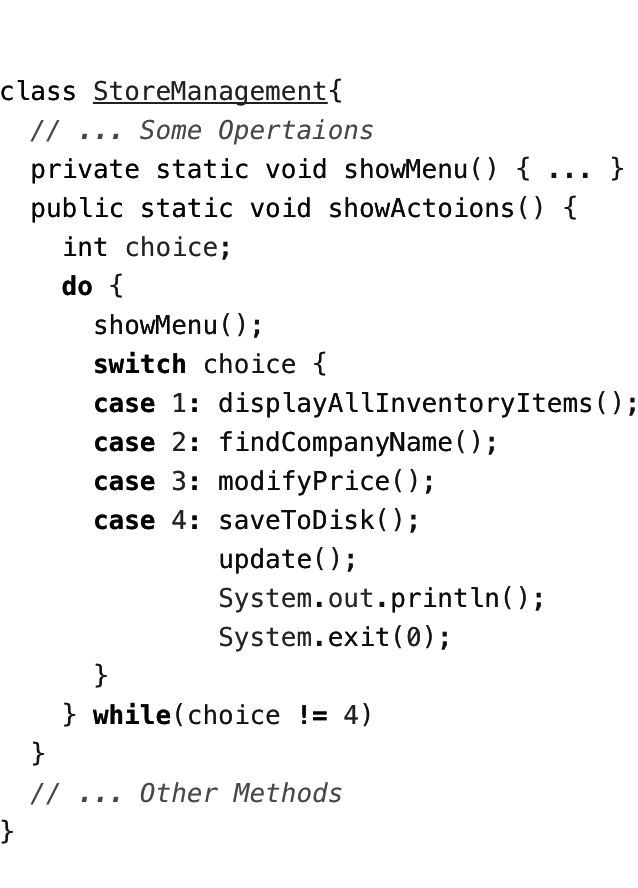
\includegraphics[width=0.45\linewidth]{1.png}}
\label{subfig:before}
}
\subfloat[After `extract method'][After `extract method']{
\fbox{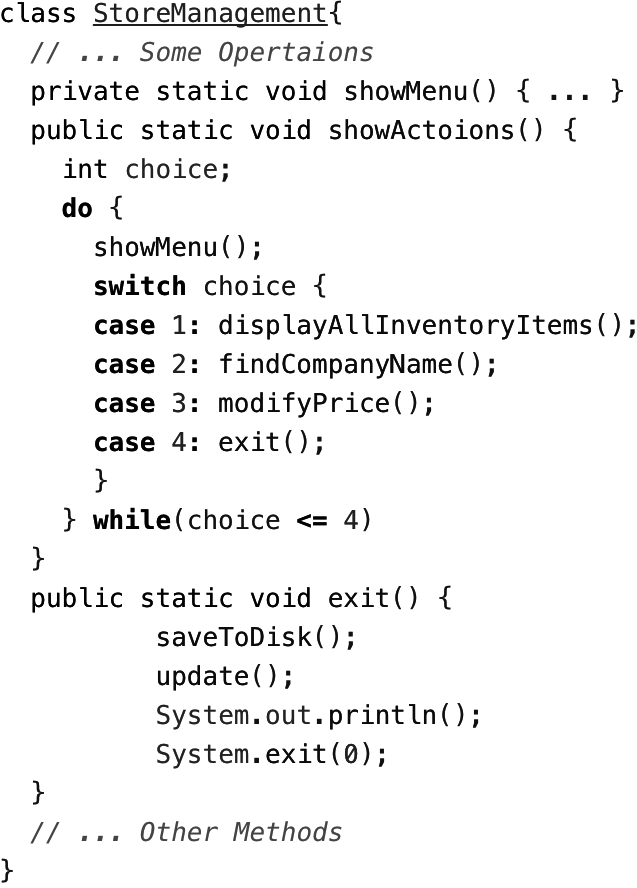
\includegraphics[width=0.45\linewidth]{2.png}}
\label{subfig:after}
}

\caption{An example of how developers might use XTREE to reduce software defects.}
\label{fig:motivating_example}
\end{figure}

On the other hand, quality planning generates a concrete set of actions that can be taken (as precautionary measures) to significantly reduce the likelihood of future defects.

For a formal definition of plans, consider a defective test example $Z$, a planner
proposes a plan ``$\Delta$'' to adjust attribute $Z_j$ as follows:
{\small\[
\forall \delta_j \in \Delta : Z_j = 
\begin{cases}
   Z_j \pm \delta_j& \text{if $Z_j$ is numeric}\\
  \delta_j       & \text{otherwise}
\end{cases}
\]}
The above plans are described in terms of a range of numeric values. In this case, they represent an increase (or decrease) in some of the static code metrics of \fig{static_metrics}. However, these numeric ranges in and of themselves may not very informative. It would be beneficial to offer a more detailed report on how to go about implementing these plans. For example, to (say) simplify a large bug-prone method, it may be useful to suggest to a developer to reduce its size (e.g., by splitting it across two simpler functions).


In order to operationalize such plans, developers need some guidance on what to change in order to achieve the desired effect. 
There are two ways to generate that guidance.
One way is to is to use a technique
% reverse engineer their recommendation (which are in the form of a range numeric range) into specific actions that will improve the quality of their designs. There has been a number of recent research by the SE community~\cite{stroggylos2007, du2006study, kataoka2002, bryton2009}, including one of our previous work~\cite{krishna2017less}, that attempt to tackle this very issue. Stroggylos \& Spinellis~\cite{stroggylos2007} studied the impact of CK-metrics to assert if performing reorganization was useful in reducing bugs and improving software quality, they reported a strong correlation between these metrics and software quality. Du Bois~\cite{du2006study} conducted a study that explored coupling and cohesion metrics and reported similar findings. Elish \& Alshayeb~\cite{elish2011, elish2012} conducted a systematic study to categorize code reorganization procedures in terms of their measurable effect on software quality attributes. Their studies showed how each reorganization action would impact several of the CK-metrics. 
% Although these and other similar studied were enlightening in that they demonstrated the strong correlation between static code metrics and the reorganization, a major shortcoming of these approaches is that they left much of the decision making to the developers. Numerous recent studies challenge this approach. Consider the findings of Devanbu et al.~\cite{devanbu2016belief}, who, after examining responses from 564 Microsoft developers around the world, showed that the some of the most ardent beliefs held by developers must now be carefully re-examined in the face of new empirical evidence. This work is response to these and other similar criticisms. The remainder of this section provide an example of how our proposed method addresses this issue.
% Our framework attempts to automate the process of decision making by reflecting on past releases of the software projects.
% To do this, we adopt two strategies, 
% the first of which was 
used by Nayrolles et al.~\cite{nayrolles2018clever} at MSR 2018. In that approach, we look through the developer's own history to find old examples where they have made the kinds of changes recommended by the plan. 

When that data is not accessible, another way to operationalize plans is via 
 guidance from the literature. Many papers have
discussed how code changes adjust
static code metrics~\cite{stroggylos2007, du2006study, kataoka2002, bryton2009, elish2011, elish2012}.

\fig{motivating_example}(b) shows a summary of
that research. 
For example, in \fig{motivating_example}, say a planner has recommended the changes shown in \fig{motivating_example}(a). Then, we use \ref{fig:motivating_example}\protect\subref{subfig:actions} to look-up possible actions developers may take, there we see that performing an ``extract method'' operation may help alleviate certain defects (this is highlighted in {\colorbox{lightgray}{gray}}). In \ref{fig:motivating_example}\protect\subref{subfig:before} we show a simple example of a class where the above operation may be performed. In \ref{fig:motivating_example}\protect\subref{subfig:after}, we demonstrate how a developer may perform the ``extract method''. 


 
We say that \fig{motivating_example} is an example of {\em code-based planning} where the goal is to change a code base in order to improve that code in some way. The rest of this section discusses other kinds of planning.

\subsection{Other Kinds of Planning}
\label{sect:planners}
Planning is extensively explored in artificial intelligence research. There, it usually refers to generating a sequence of actions that enables an \textit{agent} to achieve a specific \textit{goal}~\cite{norvig}. This can be achieved by classical search-based problem solving approaches or logical planning agents. Such planning tasks now play a significant role in a variety of demanding applications, ranging from controlling space vehicles and robots to playing the game of bridge~\cite{ghallab04}. Some of the most common planning paradigms include: (a) classical planning~\cite{wooldridge95}; (b) probabilistic planning~\cite{Bel, altman99, guo2009}; and (c) preference-based planning~\cite{son06, baier09}. Existence of a model precludes the use of each of these planning approaches. This is a limitation of all these planning approaches since not every domain has a reliable model. 



Apart from {\em code-based planning}, we know of at least two other kinds of planning research in SE. Each kind is distinguishable by {\em what} is being changed.
\bi
\item
In {\em test-based planning}, some optimization is applied to reduce the number of tests required to achieve to a certain goal or the time taken before tests yield interesting results~\cite{tallam2006concept, yoo2012regression, blue2013interaction}.
\item
In {\em process-based planning} some search-based optimizer is applied to a software process model to infer high-level business plans about software projects. Examples of that kind of work include our own prior studies combining simulated annealing with the COCOMO models or Ruhe et al.'s work on next release planning in requirements engineering~\cite{ruhe2003quantitative, ruhe2010product}. 
\ei
In software engineering, the planning problem translates to proposing changes to software artifacts. These are usually a hybrid task combining probabilistic planning and preference-based planning using search-based software engineering techniques~\cite{Harman2009, Harman2011}. These search-based techniques are evolutionary algorithms that propose actions guided by a fitness function derived from a well established domain model. Examples of algorithms used here include GALE, NSGA-II, NSGA-III, SPEA2, IBEA, MOEA/D, etc.~\cite{krall2015gale, deb00a, zit02, zit04, deb14, Cui2005a, zhang07:TEC}. 
As with traditional planning, these planning tools all require access to some trustworthy models that can be used to explore some highly novel examples. In some software engineering domains there is ready access to such models which can offer assessment of newly generated plans. Examples of such domains within software engineering include automated program repair~\cite{Weimer2009, Goues12, LeGoues2015}, software product line management~\cite{sayyad13, metzger14, henard15}, automated test generation~\cite{andrews07, andrews10}, etc. 

However, not all domains come with ready-to-use models. For example, consider all the intricate issues that may lead to defects in a product. A model that includes {\em all} those potential issues would be very large and complex. Further, the empirical data required to validate any/all parts of that model can be hard to find.
Worse yet, our experience has been that accessing and/or commissioning a model can be a labor-intensive process.
For example, in previous work~\cite{me07f} we used models developed by Boehm's group at the University of Southern California.
Those models took as inputs project descriptors to output predictions of development effort, project risk, and defects.
Some of those models took decades to develop and mature (from 1981~\cite{boehm81} to 2000~\cite{boehm00b}). 
Lastly, even when there is an existing model, they can require constant maintenance lest they become out-dated. Elsewhere, we have described our extensions to the USC models to enable reasoning about agile software developments. It took many months to implement and certify those extensions~\cite{me09i, me09j}. The problem of model maintenance is another motivation to look for alternate methods that can be quickly and automatically updated whenever new data becomes available.

In summary, for domains with readily accessible models, we recommend
the kinds of tools that are widely used in the search-based
software engineering community such as GALE, NSGA-II, NSGA-III, SPEA2, IBEA, particle swarm optimization, MOEA/D, etc. In other cases where this is not an option, we propose the use of data mining approaches to create a quasi-model of the domain and make of use observable states from this data to generate an estimation of the model. Examples of such a data mining approaches are described below.
These include five methods described in the rest of this section: XTREE, BELLTREE and the approaches of 
Alves et al.~\cite{alves}, Shatnawi~\cite{shatnawi}, and Oliveira et al.~\cite{oliveira} 

\begin{figure}[!b]
\small
\centering
\resizebox{1\linewidth}{!}{
\begin{tabular}{|p{\linewidth}|} \hline
\begin{minipage}{\linewidth}
\vspace{0.1cm}
\small
{\bf \fig{xtree}.A: Using XTREE}

Using the training data, construct a decision tree. For each test item, find the {\em current} leaf: take each test instance, run it down to a leaf in the decision tree.  
After that,	find the {\em desired} leaf:
\begin{itemize}[leftmargin=3mm]
\item Starting at {\em current}, ascend the tree levels;
\item Identify {\em sibling} leaves; i.e. leaf clusters that can be reached from level $lvl$ that are not same as {\em current}
\item Find the {\em better} siblings; i.e. those with a {\em score} (\#defects) less than $\gamma=0.5$ times the score of {\em current} branch. 
If none found, then repeat for $lvl += 1$. Also, return no plan if the new $lvl$ is above the root. 
\item  Return the {\em closest} better sibling to the {\em current}.
\end{itemize}
Also, find the {\em delta}; i.e. the set difference between conditions in the decision tree branch to {\em desired} and {\em current}. To find that delta: (1)~for discrete attributes, delta is the value from {\em desired}; (2)~for  numerics, delta is the numeric difference; (3)~for numerics  discretized into ranges, delta is a random number selected from the low and high boundaries of the that range. Finally, return the delta as the plan for improving the test instance.\\
\end{minipage}
\begin{minipage}{\linewidth}
\textbf{\fig{xtree}.B: A sample decision tree.\\}
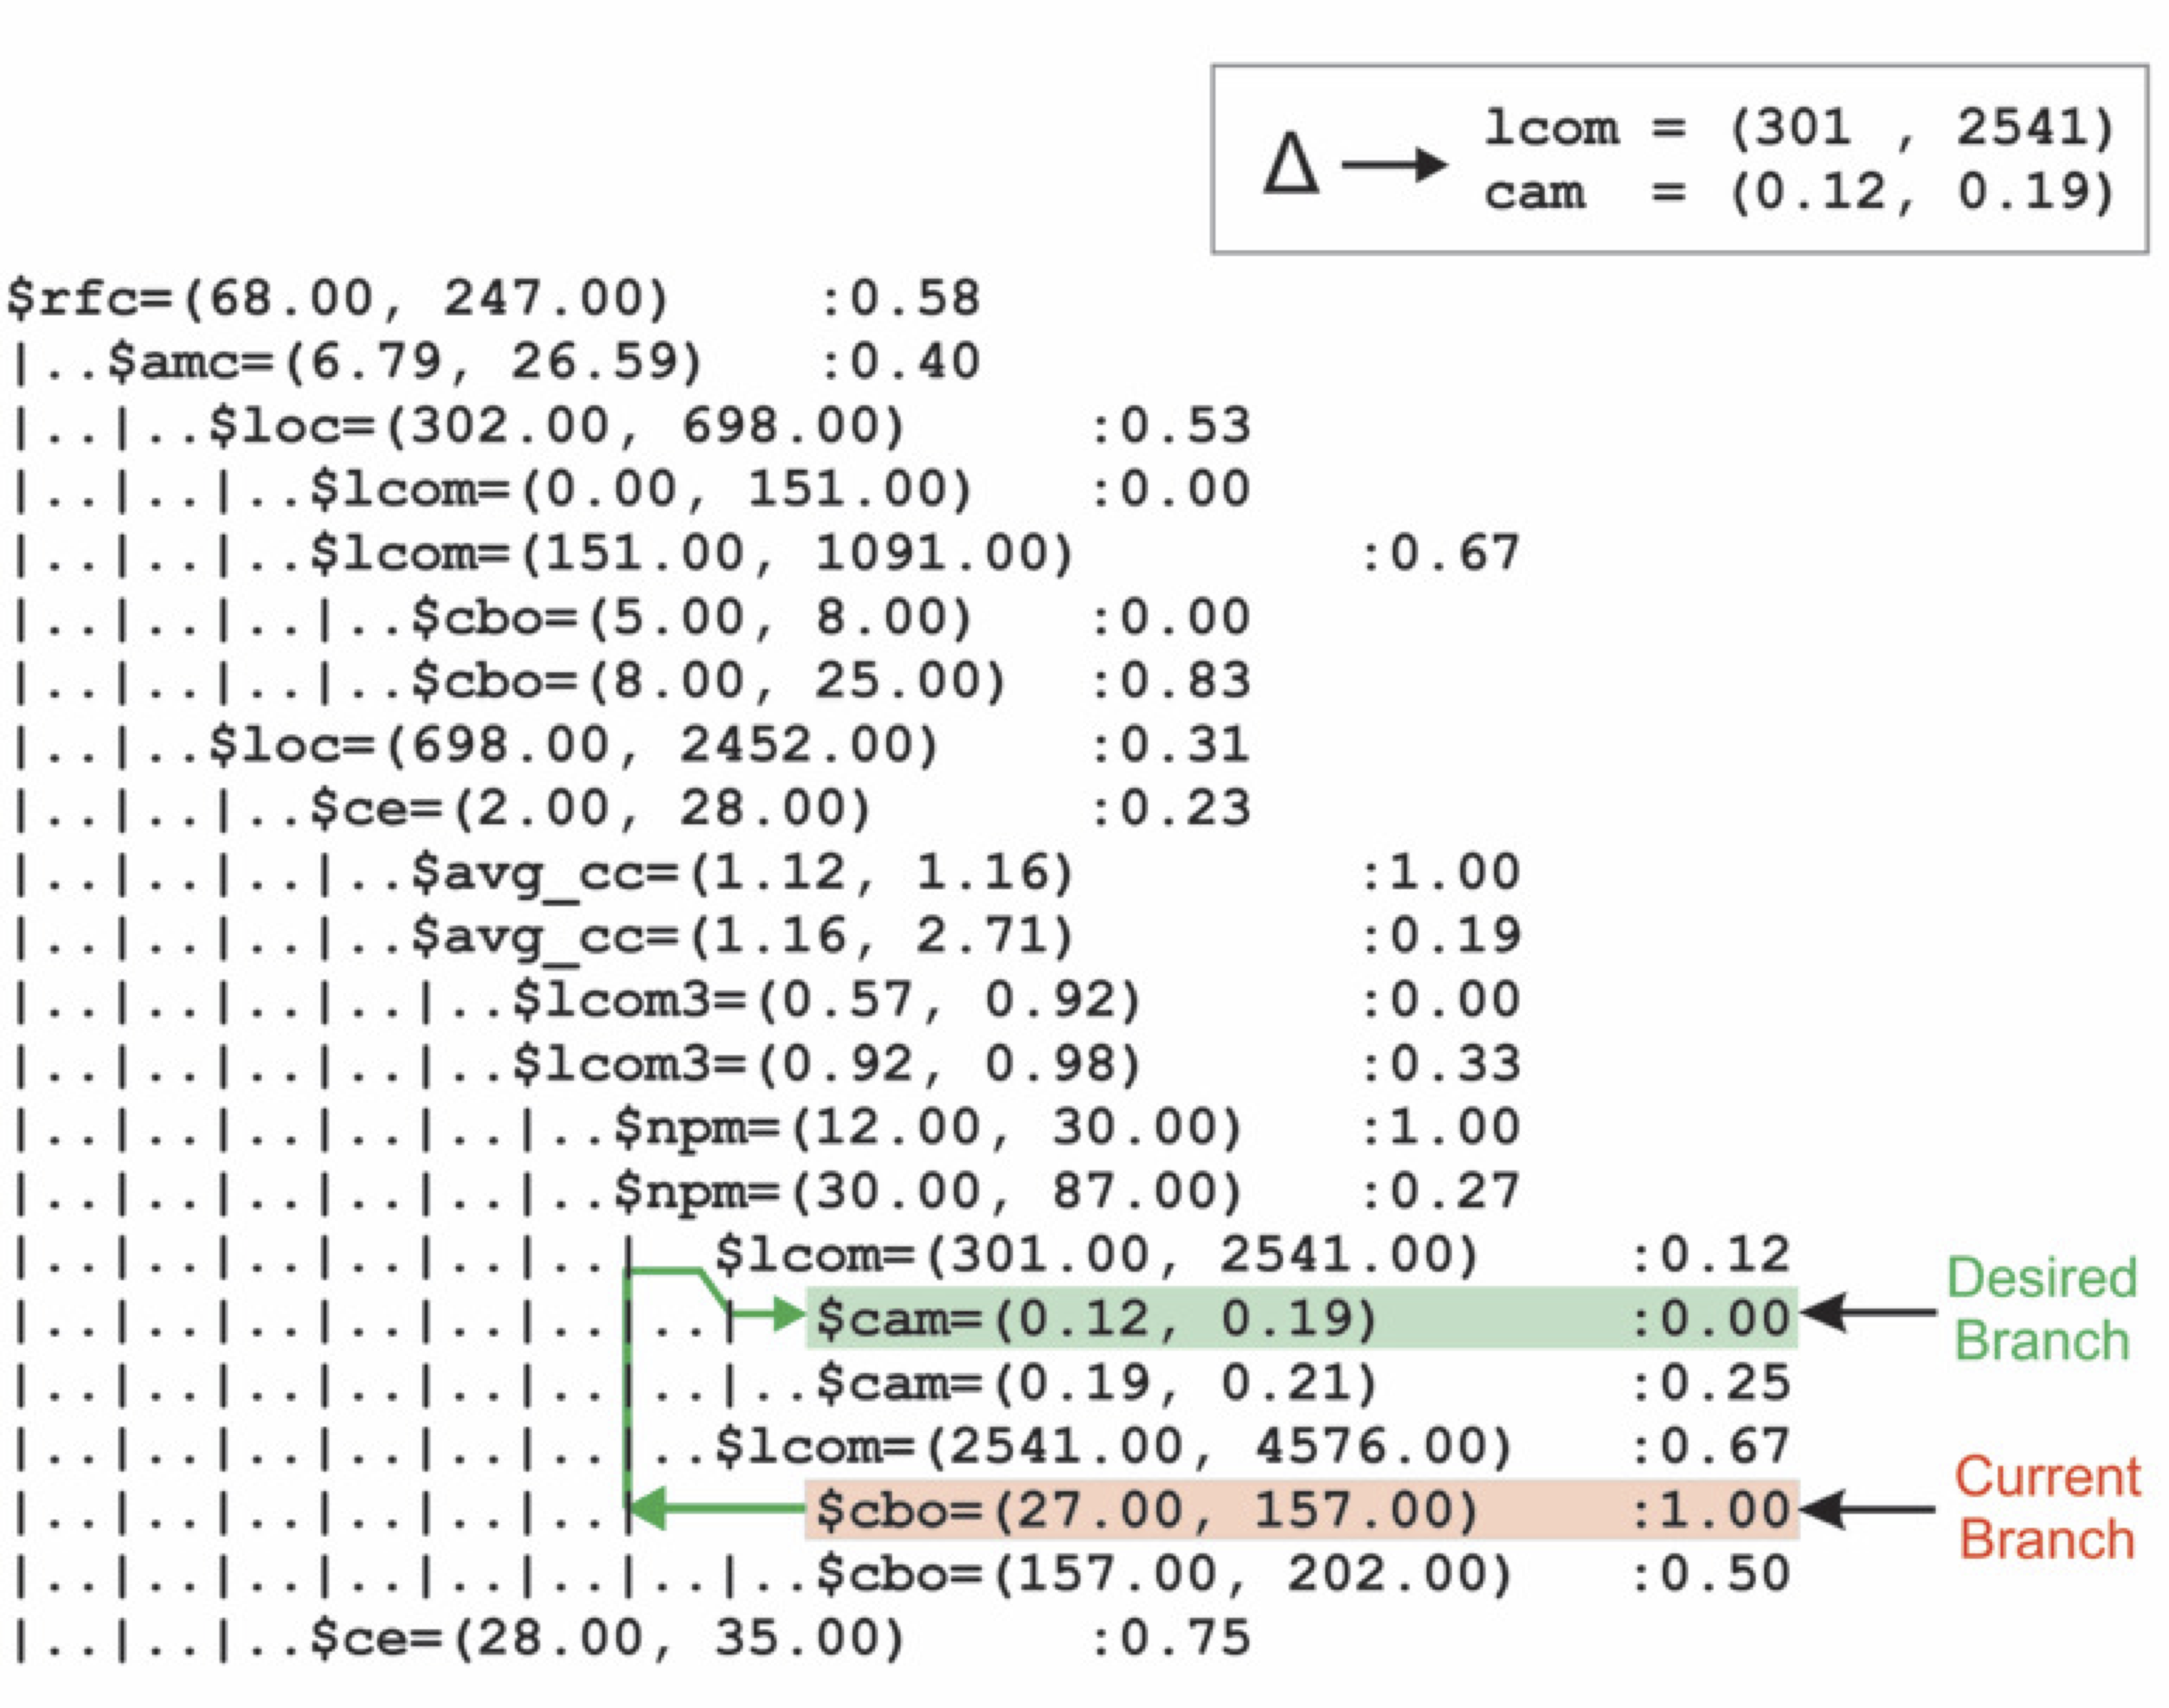
\includegraphics[width=0.99\linewidth]{XTREE_samp.png}
\end{minipage}\bigstrut\vspace{0.1cm}\\\hline
\end{tabular}}
\caption{Generating thresholds using XTREE.}\label{fig:xtree}
\end{figure}

\subsubsection{Within-Project Planning With XTREE}
\label{sect:XTREE}


XTREE builds a decision tree, then generates
plans by contrasting the differences between two branches:
(1)~the current branch; (2)~the desired branch.
XTREE uses a supervised regression tree algorithm that is constructed on discretized values OO metrics (we use Fayyad-Irani discretizer~\cite{fi}). Next, XTREE builds plans from the branches of the tree as follows, for every test instance, we ask:
\be
\item
Which {\em current} branch matches the test instance?
\item Which {\em desired} branch would the test want to emulate?
\item What are the {\em deltas} between current and desired? 
\ee
See \fig{xtree} for an example of how plans are generated using these three questions.
See \fig{motivating_example} for details on how these plans translate back to changes in the code.

\subsubsection{Cross-project Planning with BELLTREE}
\label{sect:CPXTREE}

Many methods have been proposed for transferring data or lessons
learned from one project to another, for examples see~\cite{Nam2013, Nam2015, jing15, kocaguneli2011find, kocaguneli2012, turhan09, peters15}. Of all these, the bellwether method described here is one of the simplest.
Transfer learning with bellwethers is just a matter of calling existing
learners inside a for-loop. For all the training data from different projects $\mathcal{P, Q, R, S...}$, 
a bellwether learner conducts a round-robin experiment where a model is learned from project, then applied to all others. The {\em bellwether} is that project which generates the best performing model. The {\em bellwether effect}, states that models
learned from this bellwether performs as well as, or better than, other transfer learning algorithms. 

For the purposes of prediction, we have shown previously that bellwethers are remarkably
effective for many different kinds of SE tasks such as (i)~defect prediction, (ii)~effort
estimation, and (iii)~detecting code smells~\cite{krishna17b}. This paper is the first to check the value of bellwethers for the purposes of planning. Note also that this paper's use of bellwethers enables us to generate plans from different data sets from across different projects. This represents a novel and significant extension to our previous work~\cite{krishna17a} which was limited to the use of datasets from within a few projects.



BELLTREE extends the three bellwether operators defined in our previous work~\cite{krishna17b} on bellwethers: DISCOVER, PLAN, VALIDATE. That is:~ 
\be
  \item DISCOVER: {\em Check if a community has bellwether.} 
  This step is similar to our previous technique used to discover bellwethers~\cite{krishna16}. We see if standard data miners can predict for the number of defects, given the static code attributes. This is done as follows:~ 
  \bi 
  \item
  For a community $C$ obtain all pairs of data from
  projects $\mathcal{P, Q, R, S...}$ such that $x, y \in C$;
  \item
  Predict for defects in $y$ using a quality predictor learned from data taken from $x$;
  \item
  Report a bellwether if one $x$ generates consistently high predictions in a majority of $y \in C$.
  \ei
  \item PLAN: {\em Using the bellwether, we generate plans that can improve a new project.} That is, 
  having learned the bellwether on past data, we now construct a decision tree similar to within-project XTREE. We then use the same methodology to generate the plans.
  \item VALIDATE: {\em Go back to step 1} if the performance statistics seen during PLAN fail to generate useful actions.
  \ee
  



\subsubsection{Alves}

Looking through the SE literature, we can see researchers have proposed three other methods  analogous to XTREE planning.
Those other methods are proposed by Alves et al.~\cite{alves} (described in this section) plus those of Shatnawi~\cite{shatnawi}
and Oliveira et al.~\cite{oliveira} described below.

Alves et al.~\cite{alves} proposed an unsupervised approach
that uses the underlying statistical 
distribution and scale of the OO metrics. It works by first weighting each metric value according to the source lines of 
code (SLOC) of the class it belongs to. All the weighted metrics are then normalized by the sum of all weights for the system. The normalized metric values are ordered in an ascending fashion (this is
equivalent a density function, where the x-axis represents 
the weight ratio (0-100\%), and the y-axis the metric scale).

Alves et al. then select a percentage value (they suggest 70\%) which 
represents the ``normal'' values for metrics. The metric threshold, then, 
is the metric value for which 70\% of the classes fall below. The 
intuition is that the worst code has outliers beyond 70\% of the normal 
code measurements i.e., they state that the risk of there existing a defect 
is moderate to high when the threshold value of 70\% is exceeded.

Here, we explore the correlation between the code metrics 
and the defect counts with a univariate logistic regression and reject 
code metrics that are poor predictors of defects (i.e.  those with $p > 
0.05$). For the remaining metrics, we obtain the threshold ranges which are denoted by $[0, 70\%)$ ranges for each metric. The plans would then involve reducing these metric range to lie within the thresholds discovered above.

\subsubsection{Shatnawi}

Shatnawi~\cite{shatnawi} offers a different alternative Alves et al by using VARL (Value of Acceptable Risk Level). This method was initially proposed by Bender~\cite{bender99} for his epidemiology studies. This approach uses two constants ($p_0$ and $p_1$) to compute the thresholds, which Shatnawi recommends to be set to $p_0=p_1=0.05$. Then using a univariate binary logistic regression three coefficients are learned:
$\alpha$ the intercept constant;
$\beta$ the coefficient for maximizing log-likelihood;
and $p_0$ to 
measure how well this model predicts for defects. (Note: the univariate 
logistic regression was conducted comparing metrics to defect counts. Any 
code metric with $p>0.05$ is ignored as being a poor defect predictor.)

Thresholds are learned from the surviving metrics using
the risk equation proposed by Bender:
$$ \mathit{Defective\ if}\ \mathit{Metric} > \mathit{VARL}$$
$$
	\mathit{VARL} = p^{-1}(p_0) = \frac{1}{\beta }\left( {\log \left( 
		{\frac{{{p_1}}}{{1 - {p_1}}}} \right) - \alpha } \right)
$$

In a similar fashion to Alves et al., we deduce the threshold ranges as $[0, VARL)$ for each selected metric. The plans would again involve reducing these metric range to lie within the thresholds discovered above.

\subsubsection{Oliveira}
Oliveira et al. in their 2014 paper offer yet another alternative to absolute threshold methods discussed above~\cite{oliveira}. Their method is still unsupervised, but they propose complementing the threshold by a second piece of information called the \textit{relative threshold}. This measure denotes the percentage of entities the upper limit should be applied to. These have the following format:
\[p\%\ of\ the\ entities\ must\ have\ M\leq k\]
Here, $M$ is an OO metric, $k$ is the upper limit of the metric value, and $p$ (expressed as \%) is the minimum percentage of entities are required to follow this upper limit. As an example Oliveira et al. state, ``85\% of the methods should have $CC \leq 14$. Essentially, this threshold expresses that high-risk methods may impact the quality of a system when they represent more than 15\% of the whole population''

The procedure attempts derive these values of $(p, k)$ for each metric $M$. They define a function \texttt{ComplianceRate(p, k)} that returns the percentage of system that follows the rule defined by the relative threshold pair $(p, k)$. They then define two penalty functions: (1) \texttt{penalty1(p, k)} that penalizes if the compliance rate is less than a constant $Min\%$, and (2) \texttt{penalty2(k)} to define the distance between $k$ and the median of preset $Tail$-th percentile. (Note: according to Oliveira et al., median of the tail is an idealized upper value for the metric, i.e., a value representing classes that, although present in most systems, have very high values of M). They then compute the total penalty as \texttt{penalty} = \texttt{penalty1(p, k)} + \texttt{penalty2(k)}. Finally, the relative threshold is identified as the pair of values $(p, k)$ that has the lowest total \texttt{penalty}. After obtaining the $(p, k)$ for each OO metric. As in the above two methods, the plan would involve ensuring the for every metric $M$ $p\%$ of the entities have a value that lies between $(0, k]$. 

\section{Research Methods}
\label{sect:prelim}

The rest of this paper compares XTREE and BELLTREE against  
Alves, Shatnawi, Oliveira et al. 

\subsection{Datasets}
\label{sect:data}
The defect dataset used in this study comprises a total of 38 datasets from 10 different projects taken from previous transfer learning studies. This group of data was gathered by Jureczko et al. \cite{Jureczko2010}. They recorded the number of known defects for each class using a post-release bug tracking system. The classes are described in terms of 20 OO metrics, including CK metrics and McCabes complexity metrics, see~\fig{static_metrics} for description. Since we attempt to learn plans from within the project and across projects, we explore \textit{homogeneous} transfer of plans. Homogeneity requires that the attributes (static code metrics) are the same for all the datasets and all the projects. We obtained the dataset from the SEACRAFT repository\footnote{$\text{https://zenodo.org/communities/seacraft/}$} (formerly the PROMISE repository~\cite{menzies2016promise}). For more information see~\cite{krishna16}. 



\subsection{A Strategy for Evaluating Planners}

It can be somewhat difficult to judge the effects of applying plans
to software projects. These plans cannot be assessed just by a rerun of the test suite for three reasons: (1) The defects were recorded by a post release bug tracking system. It is entirely possible it escaped detection by the existing test suite; (2) Rewriting test cases to enable coverage of all possible scenarios presents a significant challenge; and (3) It may take a significant amount of effort to write new test cases that identify these changes as they are made.

To resolve this problem, SE researchers such as
Cheng et al.~\cite{Cheng10}, O'Keefe et al.~\cite{OKeeffe08, OKeeffe07}, 
Moghadam~\cite{Moghadam2011} and Mkaouer et al.~\cite{Mkaouer14}
use a {\em verification oracle} learned separately from the primary oracle. This oracles assesses how defective the code is before and after some code changes. For their oracle, Cheng, O'Keefe, Moghadam and Mkaouer et al. use the QMOOD quality model~\cite{Bansiya02}.

A shortcoming of QMOOD is that quality models learned from other projects may perform poorly when applied to new projects~\cite{localvsglobal}. Hence,  we eschew older quality models like QMOOD and propose a verification oracle based on the  {\em overlap}.
between two sets: (1) The changes that developers made, perhaps in response to the issues raised in a post-release issue tracking system; and (2) Plans recommended by an automated planning tool such as XTREE/BELLTREE.
Using these two sources of changes, it is possible to compute the extent to which a developer's action matches that of the actions recommended by planners. This is measured using \textit{overlap}:
\begin{equation}
\mathit{Overlap} = \frac{|\mathcal{D} \cap \mathcal{P}|}{|\mathcal{D} \cup \mathcal{P}|}\times 100  
\end{equation}
\newcolumntype{M}{@{}>{\columncolor{white}[0pt][0pt]}l@{}}
\begin{figure}[!t]
\centering
% \setlength{\col}{}
\begin{minipage}{\linewidth}
\resizebox{\linewidth}{!}{%
% Table generated by Excel2LaTeX from sheet 'Sheet1'
\scriptsize \begin{tabular}{Mrrrl}
\toprule
Dataset & \multicolumn{1}{r}{Versions} & \multicolumn{1}{r}{$N$} & Bugs (\%) & Description\bigstrut\\\midrule
 Lucene & 2.2 -- 2.4 & 782  & 438 (56.01) & Information retrieval software library\bigstrut\\
 Ant   & 1.3 -- 1.7 & 1692  & 350 (20.69) & A software tool for automating\bigstrut\\
 &&&& software build processes\bigstrut\\
 Ivy   & \multicolumn{1}{r}{1.1, 1.4,2.0} & 704   & 119 (16.90) & A transitive package manager\bigstrut\\
 Jedit & \multicolumn{1}{r}{4.0 -- 4.3} & 1749  & 303 (17.32) & A free software text editor\bigstrut\\
 Poi   & \multicolumn{1}{r}{1.5, 2, 2.5, 3.0} & 1378  & 707 (51.31) & Java libraries for manipulating files in\bigstrut\\
 &&&& MS Office format.\bigstrut\\
 Camel & \multicolumn{1}{r}{1.0, 1.2, 1.4,1.6} & 2784  & 562 (20.19) & A framework for message-oriented middleware.\bigstrut\\
 Log4j & \multicolumn{1}{r}{1.0, 1.1,1.2} & 449   & 260 (57.91) & A Java-based logging utility.\bigstrut\\
 Velocity & \multicolumn{1}{r}{1.4, 1.5,1.6} & 639   & 367 (57.43) & A template engine to reference objects in Java.\bigstrut\\
 Xalan & \multicolumn{1}{r}{2.4, 2.5, 2.6,2.7} & 3320  & 1806 (54.40) & A Java implementation of XLST, XML, and XPath.\bigstrut\\
 Xerces & \multicolumn{1}{r}{1.0, 1.2, 1.3,1.4} & 1643  & 654 (39.81) & Software libraries for manipulating XML.\bigstrut\\\bottomrule
\end{tabular}%
}
\end{minipage}
\caption{The figure lists defect datasets used in this paper.}
\label{fig:datasets}
\end{figure}

That is, we measure  overlap using the size of the intersections divided by the size of the union of the \textit{changes}. Here $\mathcal{D}$ represents the changes made by the \textit{developers} and $\mathcal{P}$ represents the changes recommended by the \textit{planner}. Accordingly, the larger the intersection between the changes made by the developers to the changes recommended by the planner, the greater the overlap. 

\begin{figure}[!b]
\centering
\resizebox{\linewidth}{!}{
\begin{tabular}{c|ccccccccc}
& DIT & NOC & CBO & RFC & FOUT & WMC & NOM & LOC & LCOM \bigstrut\\\hline
Planner ($\mathcal{P}$) & \cellcolor[HTML]{D0D0D0}$\cdot$ & \cellcolor[HTML]{D0D0D0}$\cdot$ & $\cdot$  & \cellcolor[HTML]{D0D0D0}$+$  & $\cdot$   & \cellcolor[HTML]{D0D0D0}$+$  & \cellcolor[HTML]{D0D0D0}$+$  & \cellcolor[HTML]{D0D0D0}$+$  & \cellcolor[HTML]{D0D0D0}$+$  \bigstrut\\
Developer ($\mathcal{D}$) & \cellcolor[HTML]{D0D0D0}$\cdot$ & \cellcolor[HTML]{D0D0D0}$\cdot$ & $-$  & \cellcolor[HTML]{D0D0D0}$+$  & $-$   & \cellcolor[HTML]{D0D0D0}$+$  & \cellcolor[HTML]{D0D0D0}$+$  & \cellcolor[HTML]{D0D0D0}$+$  & \cellcolor[HTML]{D0D0D0}$+$  \\
\end{tabular}}\\
\[
Overlap = \frac{|\mathcal{D} \cap \mathcal{P}|}{|\mathcal{D} \cup \mathcal{P}|}\times 100 = \frac{7}{9}\times100 = 77.77\%
\]
\caption{A simple example of computing overlap. Here a `$+$' represents an \textit{increase}, a `$-$' represents a \textit{decrease}, and a `$\cdot$' represents \textit{no-change}. Columns shaded in \colorbox{lightgray}{gray} indicate a match between developer's change and the recommendation made by a planner.}
\label{fig:overlap_example}
\end{figure}

As an example, consider \fig{overlap_example}; there we have 2 sets of changes: (1) Changes made by developers ($\mathcal{D}$), and (2) Changes recommended by the planner ($\mathcal{P}$). In each case we have 3 possible actions for every metric: (1) Make no change (`$\cdot$'), (2) Increase (`$+$'), and (3) Decrease (`$-$'). The intersection of the changes represents the number of times the actions taken by the developers is the same as the actions recommended by the planner. This the above example, the intersection, $\mathcal{D}\cap\mathcal{P}=7$, out of a total of $\mathcal{D}\cup\mathcal{P}=9$ possible actions. This leads to $Overlap=\frac{7}{9}\times100=77.77\%$.





\subsubsection{The \ktest}

Measuring overlap as described in the previous section only measures the extent to which the recommendations made by planning tools match those undertaken by the developers. 
Note that overlap does not measure the \textit{quality} of the recommendation. Specifically, it does not tell us what the impact of making those changes would be to future releases of a project. Therefore, it is necessary to augment the overlap with a measure of how many defects are reduced as a result of making the changes. 


For this purpose, we propose the \ktest. Given a project $\mathcal{P}$ with versions $v\in\{\mathcal{P}_i, \mathcal{P}_j, \mathcal{P}_k\}$ ordered chronologically (that is, version $i<j<k$ in terms of release dates), we divide  project data into three sets \textit{train}, \textit{test}; and \textit{validation}
which are used as follows:
\be
\item First, train the planner on version $\mathcal{P}_i$. Note: this could either be data that is either a previous release (version i), or it could be data from the bellwether dataset. 
\item Next, use the planner to generate plans to reduce defects for version $\mathcal{P}_j$.
\item Finally, on version $\mathcal{P}_k$, we measure the OO metrics for each class in $\mathcal{P}_j$, then we (a) measure the overlap between plans recommended by the planner and the developer's actions; (b) count the number of defects reduced/increased when compared to the previous release as a result of implementing these plans.
\ee

As the outcome of the {\ktest}~we obtain the number of defects (increased or decreased) and the extent of overlap (from 0\% to 100\%). These two measures enable us to plot the operating characteristic curve for the planners (referred to henceforth as planner effectiveness curve). The operating characteristic (OC) curve depicts the effectiveness of a planner with respect to its ability to reduce defects. The OC curve plots the overlap of developer changes with the planner's recommendations versus the number of defects reduced. A sample curve for one of our datasets is shown in \fig{report_sample}.

For each of the datasets with versions $i, j, k$ we (1)~train the planner on version $i$; (2) deploy the planner to recommend plans for version $j$; and (3) validate plans for version $j$. Following this, we plot the ``planner effectiveness curve''. Finally, as in \fig{report_sample}, we compute the area under the planner effectiveness curve (AUPEC) using simpsons rule~\cite{Burden:1988}.


% In addition to this, we count the frequency with which a certain code metric is changed. This is expressed as percentage change, measured using the following equation:
% \begin{equation}
% 	\label{eq:change}
% 	\small
% 	Change=\frac{\mathit{\#times\ M\ changed}}{\mathit{\#test\ cases}}\times100\%~~~~\forall M \in OO\ Metrics
% \end{equation}


 
\begin{figure}[t!]
\small
\centering
\begin{tabular}{|p{0.95\linewidth}|} \hline
%\vspace{0.02cm}
%\textbf{Planner Effectiveness Curve:}
%\textbf{Defect Decreased (Increased) vs. Overlap Curve}
\begin{center}
    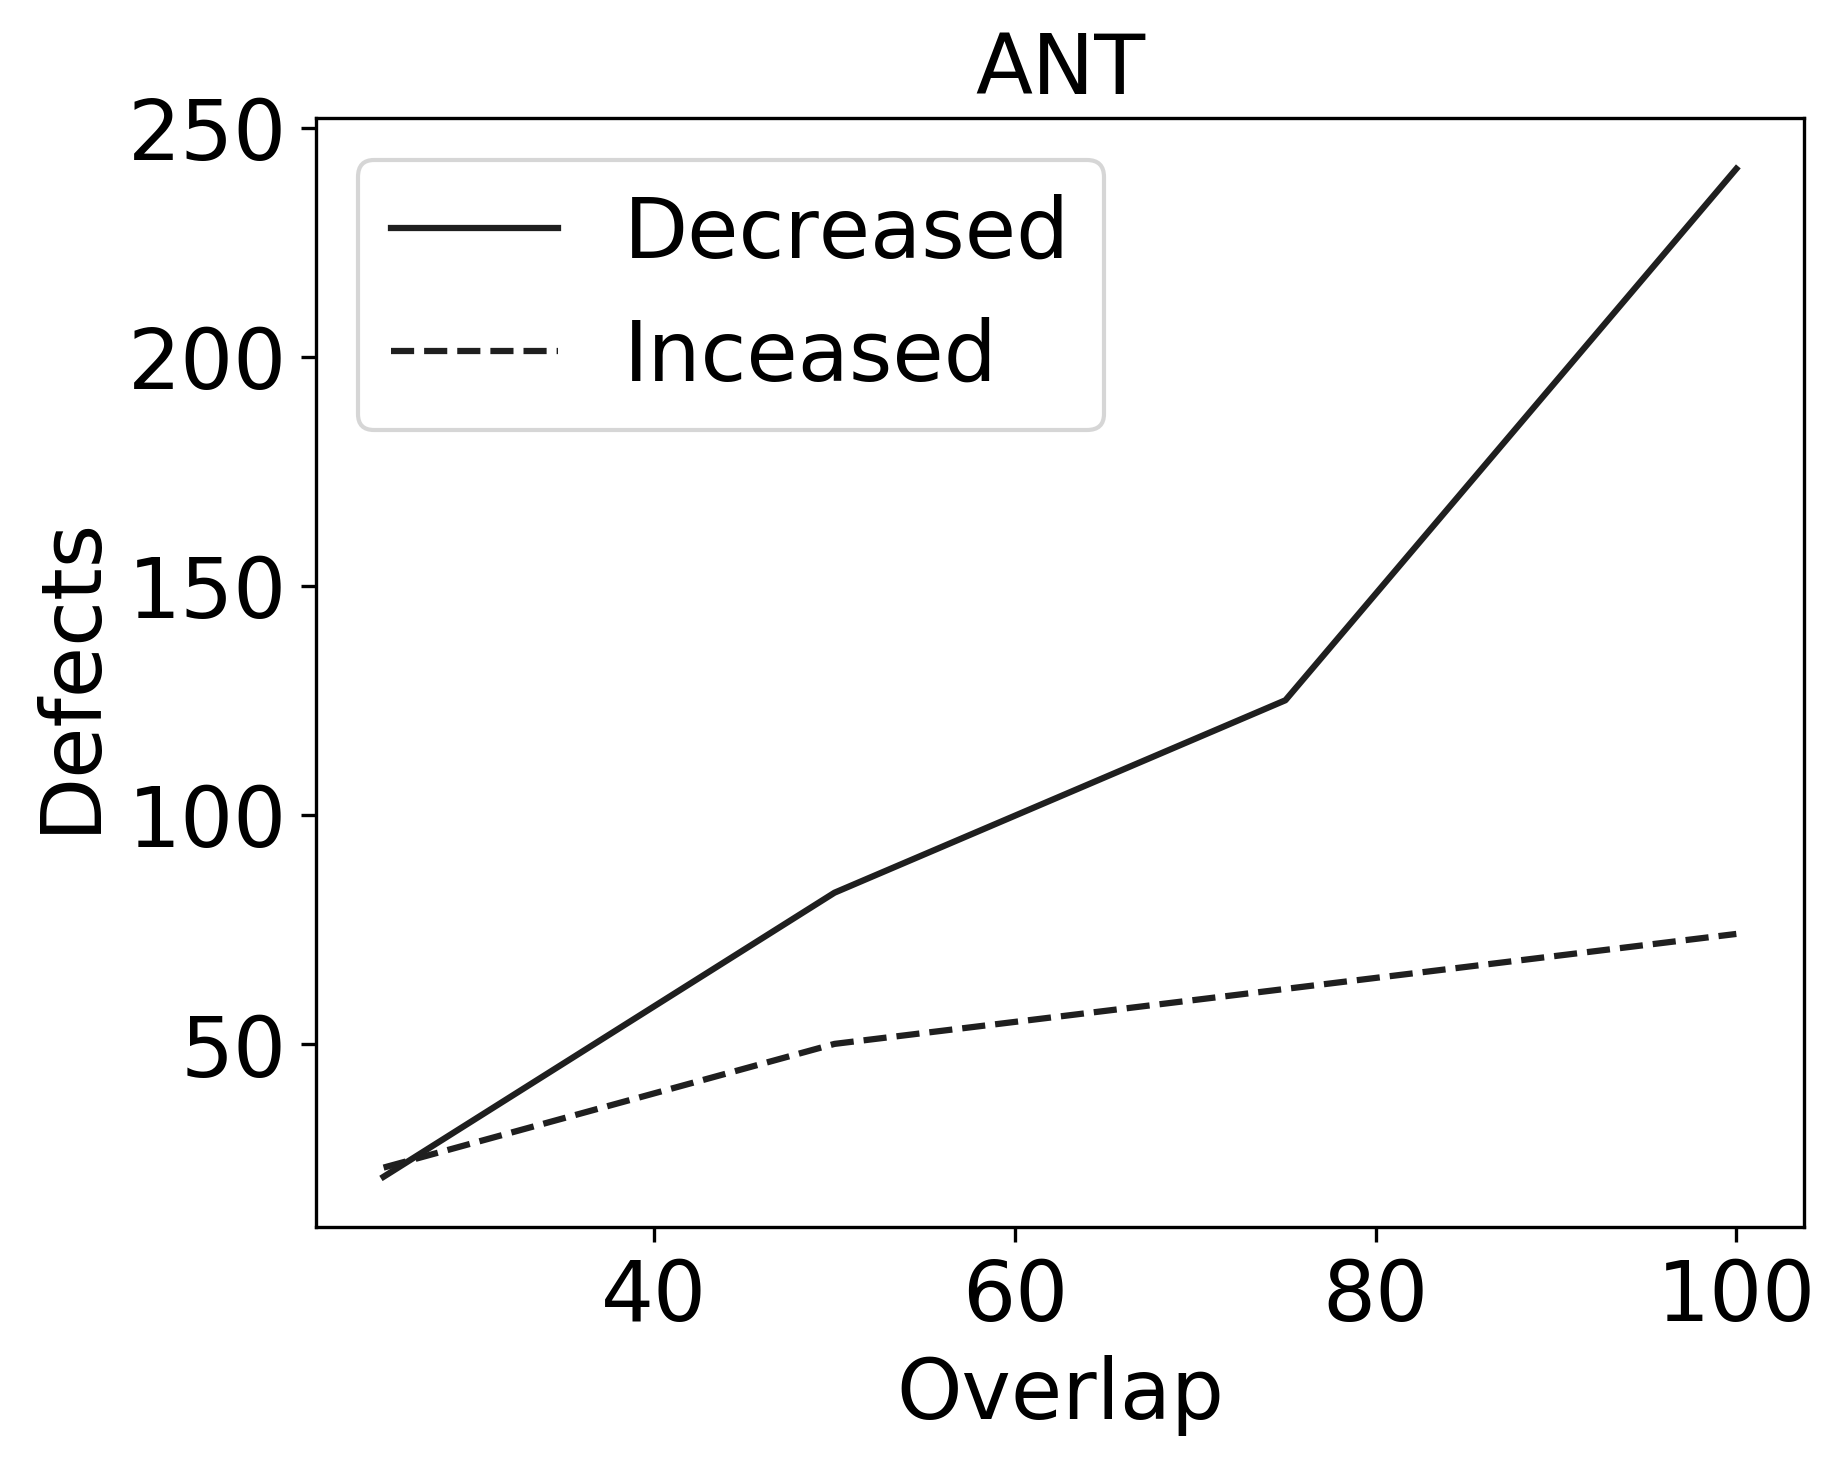
\includegraphics[width=0.7\linewidth]{sample_ant.png}
\end{center}
\[
\mathit{AUPEC} = \int_{0}^{1} f(x) \, dx \hfill
\]
\[\approx \tfrac{\Delta x}{3}\left(f(x_0) + 4f(x_1)+2f(x_2)+\cdots+4f(x_{n-1}) + f(x_{n})\right)
\]
Here, the variable $x$ represents the overlap between plans and developer changes
and  $f(x)$ represents the number of defects reduced as result of the overlap.\\

We should interpret AUPEC as follows:
\begin{enumerate}
    \item \textit{Defects Reduced:}
  AUPEC is always greater than zero and 
    \textit{larger values} of AUPEC point to \textit{more defects reduced} with increasing overlap.
    
        \item \textit{Defects Increased:}  AUPEC is still always greater than zero
        and \textit{smaller values} of AUPEC point to \textit{less defects increased} with increasing overlap.
   
\end{enumerate}
In the above plot, we show an example of XTREE on Ant. We see that the more developers used our plans (and moved right across the x-axis), then subsequent changes to the code removed far more defects than it added.  

Note: Since the actual number of defects vary from one project to another, we report the AUPEC score as a percentage of theoretical best. The theoretical best for AUPEC for defects reduced will be 100\% and 0\% for defects increased.
 
% On the other hand, in the right-hand-side figure,  when we look at defects \textit{increased}, XTREE still has a larger number of defects increased than other planners; but, the number of defects reduced in comparison to defects increased is significantly larger. Therefore, overall, we may assert that XTREE is a better planner.
\\\hline
\end{tabular}
\caption{ AUPEC = Area Under Planner Effectiveness Curve.}
\label{fig:report_sample}
\end{figure}

\begin{figure*}[!htbp]
\centering
\subfloat[][Within Project]{
\resizebox{0.66\linewidth}{!}{
\begin{tabular}{rl|rl|rl|rl|rr|}
&            & \multicolumn{2}{c|}{\begin{sideways}XTREE\end{sideways}}                                                                                                 & \multicolumn{2}{c|}{\begin{sideways}Alves\end{sideways}} & \multicolumn{2}{c|}{\begin{sideways}Shatnawi~~~~\end{sideways}} & \multicolumn{2}{c|}{\begin{sideways}Oliveira\end{sideways}} \bigstrut\\
&            & $\bigtriangledown$                                                                     & $\bigtriangleup$                                              & $\bigtriangledown$          & $\bigtriangleup$         & $\bigtriangledown$           & $\bigtriangleup$           & $\bigtriangledown$           & $\bigtriangleup$           \bigstrut\\ \hline
\multicolumn{1}{l|}{}                         & ant-1      & \cellcolor[HTML]{C0C0C0}61$^{\dagger\ddagger}$                        & 9                                                & 41           & 9           & 40            & 10            & 19            & 0             \bigstrut[t]\\
\multicolumn{1}{l|}{}                         & ant-2      & \cellcolor[HTML]{C0C0C0}{\color[HTML]{000000} 42$^{\dagger}$} & 21                                               & 35           & 16          & 33            & 15            & 7             & 5             \\
\multicolumn{1}{l|}{\multirow{-3}{*}{Ant}}    & ant-3      & \cellcolor[HTML]{C0C0C0}{\color[HTML]{000000} 53$^{\dagger}$} & 24                                               & 33           & 15          & 33            & 16            & 21            & 9             \bigstrut[b]\\ \hline
\multicolumn{1}{l|}{}                         & camel-1    & \cellcolor[HTML]{C0C0C0}{\color[HTML]{000000} 45$^{\dagger}$} & 4                                                & 24           & 1           & 22            & 3             & 19            & 3             \bigstrut[t]\\
\multicolumn{1}{l|}{\multirow{-2}{*}{Camel}}  & camel-2    & \cellcolor[HTML]{C0C0C0}{\color[HTML]{000000} 37$^{\dagger}$}                       & 7                                                & 27           & 4           & 26            & 1             & 8             & 3             \bigstrut[b]\\ \hline
\multicolumn{1}{l|}{Ivy}                      & ivy-1      & \cellcolor[HTML]{C0C0C0}{\color[HTML]{000000} 29$^{\dagger}$}                       & 9                                                & 24           & 8           & 25            & 8             & 5             & 1             \bigstrut\\ \hline
\multicolumn{1}{l|}{}                         & jedit-1    & \cellcolor[HTML]{C0C0C0}{\color[HTML]{000000} 42$^{\dagger}$} & 13                                               & 26           & 7           & 26            & 7             & 16            & 6             \bigstrut[t]\\
\multicolumn{1}{l|}{}                         & jedit-2    & \cellcolor[HTML]{C0C0C0}{\color[HTML]{000000} 59$^{\dagger}$} & 5                                                & 35           & 3           & 35            & 3             & 24            & 2             \\
\multicolumn{1}{l|}{\multirow{-3}{*}{Jedit}}  & jedit-3    & \cellcolor[HTML]{C0C0C0}{\color[HTML]{000000} 73$^{\dagger}$} & 1                                                & 51           & 1           & 49            & 1             & 22            & 0             \bigstrut[b]\\ \hline
\multicolumn{1}{l|}{Log4j}                    & log4j-1    & 16$^{\dagger\ddagger}$                                                                      & \cellcolor[HTML]{C0C0C0}41 & 2            & 22          & 3             & 21            & 11            & 17            \bigstrut\\ \hline
\multicolumn{1}{l|}{Lucene}                   & lucene-1   & \cellcolor[HTML]{C0C0C0}57$^{\dagger}$                        & 41                                               & 8            & 17          & 8             & 18            & 46            & 24            \bigstrut\\ \hline
\multicolumn{1}{l|}{}                         & poi-1      & 22$^{\dagger}$                                                                      & \cellcolor[HTML]{C0C0C0}52 & 18           & 45          & 17            & 45            & 4             & 8             \bigstrut[t]\\
\multicolumn{1}{l|}{\multirow{-2}{*}{Poi}}    & poi-2      & \cellcolor[HTML]{C0C0C0}63$^{\dagger\ddagger}$                        & 14                                               & 4            & 6           & 5             & 5             & 58            & 8             \bigstrut[b]\\ \hline
\multicolumn{1}{l|}{Velocity}                 & velocity-1 & \cellcolor[HTML]{C0C0C0}43$^{\dagger}$                        & 4                                                & 7            & 1           & 6             & 2             & 33            & 83            \bigstrut\\ \hline
\multicolumn{1}{l|}{}                         & xalan-1    & \cellcolor[HTML]{C0C0C0}31$^{\dagger\ddagger}$                                              & 15                                               & 10           & 8           & 9             & 8             & 19            & 6             \bigstrut[t]\\
\multicolumn{1}{l|}{\multirow{-2}{*}{Xalan}}  & xalan-2    & 54$^{\dagger}$                                                                      & \cellcolor[HTML]{C0C0C0}56 & 1            & 36          & 2             & 34            & 43            & 20            \bigstrut[b]\\ \hline
\multicolumn{1}{l|}{}                         & xerces-1   & \cellcolor[HTML]{C0C0C0}23$^{\dagger\ddagger}$                                              & 6                                                & 17           & 4           & 5             & 6             & 6             & 2             \bigstrut[t]\\
\multicolumn{1}{l|}{\multirow{-2}{*}{Xerces}} & xerces-2   & 24$^{\dagger}$                                                                      & \cellcolor[HTML]{C0C0C0}42 & 18           & 31          & 19            & 30            & 6             & 11  \bigstrut[b]\\       
\end{tabular}}
\label{subfig:wp}}%


\subfloat[][Cross-Project]{
\resizebox{0.66\linewidth}{!}{
\begin{tabular}{|rl|rl|rl|rl|rr}
&            & \multicolumn{2}{c|}{\begin{sideways}BELLTREE\end{sideways}}                                                                                                 & \multicolumn{2}{c|}{\begin{sideways}Alves\end{sideways}} & \multicolumn{2}{c|}{\begin{sideways}Shatnawi\end{sideways}} & \multicolumn{2}{c}{\begin{sideways}Oliveira\end{sideways}} \bigstrut[b]\\
&            & $\bigtriangledown$                                                                     & $\bigtriangleup$                                              & $\bigtriangledown$          & $\bigtriangleup$         & $\bigtriangledown$           & $\bigtriangleup$           & $\bigtriangledown$           & $\bigtriangleup$           \bigstrut\\ \hline
\multicolumn{1}{|l|}{}                         & ant-1      & \cellcolor[HTML]{C0C0C0}59$^{\dagger}$                        & 9                                                & 22           & 0           & 28            & 0            & 19            & 0             \bigstrut[t]\\
\multicolumn{1}{|l|}{}                         & ant-2      & \cellcolor[HTML]{C0C0C0}{\color[HTML]{000000} 42$^{\dagger}$} & 21                                               & 8           & 5          & 9            & 6            & 7             & 5             \\
\multicolumn{1}{|l|}{\multirow{-3}{*}{Ant}}    & ant-3      & \cellcolor[HTML]{C0C0C0}{\color[HTML]{000000} 61$^{\dagger\ddagger}$} & 27                                               & 25           & 11          & 29            & 10            & 23            & 10             \bigstrut[b]\\ \hline
\multicolumn{1}{|l|}{}                         & camel-1    & \cellcolor[HTML]{C0C0C0}{\color[HTML]{000000} 48$^{\dagger\ddagger}$} & 4                                                & 27           & 3           & 37            & 4             & 21            & 3             \bigstrut[t]\\
\multicolumn{1}{|l|}{\multirow{-2}{*}{Camel}}  & camel-2    & \cellcolor[HTML]{C0C0C0}{\color[HTML]{000000} 37$^{\dagger}$}                       & 6                                                & 11           & 3           & 15            & 4             & 8             & 2             \bigstrut[b]\\ \hline
\multicolumn{1}{|l|}{Ivy}                      & ivy-1      & \cellcolor[HTML]{C0C0C0}{\color[HTML]{000000} 29$^{\dagger}$}                       & 9                                                & 5           & 1           & 2            & 1             & 5             & 1             \bigstrut\\ \hline
\multicolumn{1}{|l|}{}                         & jedit-1    & \cellcolor[HTML]{C0C0C0}{\color[HTML]{000000} 44$^{\dagger\ddagger}$} & 13                                               & 21           & 7           & 24            & 8             & 17            & 6             \bigstrut[t]\\
\multicolumn{1}{|l|}{}                         & jedit-2    & \cellcolor[HTML]{C0C0C0}{\color[HTML]{000000} 66$^{\dagger\ddagger}$} & 5                                                & 29           & 2           & 31            & 2             & 26            & 2             \\
\multicolumn{1}{|l|}{\multirow{-3}{*}{Jedit}}  & jedit-3    & \cellcolor[HTML]{C0C0C0}{\color[HTML]{000000} 73$^{\dagger}$} & 1                                                & 23           & 0           & 21            & 0             & 22            & 0             \bigstrut[b]\\ \hline
\multicolumn{1}{|l|}{Log4j}                    & log4j-1    & 13$^{\dagger}$                                                                      & \cellcolor[HTML]{C0C0C0}39 & 14            & 21          & 18             & 25            & 11            & 17            \bigstrut\\ \hline
\multicolumn{1}{|l|}{Lucene}                   & lucene-1   & \cellcolor[HTML]{C0C0C0}57$^{\dagger}$                        & 41                                               & 8            & 17          & 8             & 18            & 46            & 24            \bigstrut\\ \hline
\multicolumn{1}{|l|}{}                         & poi-1      & 22$^{\dagger}$                                                                      & \cellcolor[HTML]{C0C0C0}52 & 10           & 14          & 20            & 20            & 14             & 8             \bigstrut[t]\\
\multicolumn{1}{|l|}{\multirow{-2}{*}{Poi}}    & poi-2      & \cellcolor[HTML]{C0C0C0}47$^{\dagger}$                        & 32                                               & 15            & 18           & 18             & 22             & 13            & 17             \bigstrut[b]\\ \hline
\multicolumn{1}{|l|}{Velocity}                 & velocity-1 & \cellcolor[HTML]{C0C0C0}48$^{\dagger\ddagger}$                        & 1                                                & 53            & 4           & 81             & 5             & 39            & 3            \bigstrut\\ \hline
\multicolumn{1}{|l|}{}                         & xalan-1    & \cellcolor[HTML]{C0C0C0}34$^{\dagger\ddagger}$                                              & 15                                               & 20           & 9           & 29             & 11             & 20            & 6             \bigstrut[t]\\
\multicolumn{1}{|l|}{\multirow{-2}{*}{Xalan}}  & xalan-2    & 54$^{\dagger}$                                                                      & \cellcolor[HTML]{C0C0C0}73 & 1            & 39          & 2             & 47            & 43            & 25            \bigstrut[b]\\ \hline
\multicolumn{1}{|l|}{}                         & xerces-1   & \cellcolor[HTML]{C0C0C0}22$^{\dagger}$                                              & 5                                                & 7           & 2           & 14             & 2             & 5             & 1             \bigstrut[t]\\
\multicolumn{1}{|l|}{\multirow{-2}{*}{Xerces}} & xerces-2   & \cellcolor[HTML]{C0C0C0}54$^{\dagger\ddagger}$                                                                      & 41 & 8           & 13          & 14            & 15            & 5             & 10  \bigstrut[b]\\      
\end{tabular}}
\label{subfig:cp}}
\caption{\small{Area Under Planner Effectiveness Curve (AUPEC) obtained with the \ktest~for all planners. $\bigtriangledown$ indicates AUPEC for defects reduced and $\bigtriangleup$ indicates AUPEC for defects increased. \textit{Larger} values for $\bigtriangledown$ are preferable and \textit{smaller} values for $\bigtriangleup$ are preferable. For each row,
cells with the largest AUPEC values shaded in \colorbox{lightgray}{gray}. Note that in 14 out of 18 cases, XTREE/BELLTREE reduces far more defects than it increases. Cells labeled with ${\dagger}$ indicates the best planner for \textit{reducing} defects. Note that in all cases, XTREE/BELLTREE outperform other planners. To compare XTREE with BELLTREE, cells are labeled with ${\ddagger}$. In 5 cases XTREE is better than BELLTREE, in 7 cases BELLTREE is better than XTREE, and in 6 cases they are comparable.}}
\label{fig:results}
\end{figure*}

\section{Experimental Results}
\label{sect:results}
\subsection*{{\bf RQ1: Is within-project planning with XTREE comparatively
more effective?}}

We answer this question in two parts: (a) First, we assess the effectiveness of XTREE (using Area Under Planner Effectiveness Curve); (b) Next, we compare XTREE with other threshold based planners. In each case, we split the available data into training, testing, and validation. That is, given versions $v_1, v_2, ..., v_K$, we, 
{\em train} the planners on version $v_1$; then 
{\em generate plans} using the planners for version $v_2$;
then {\em validate} the effectiveness of those plans on $v_3$ using the \ktest.
Then,  we repeat the process by training on $v_2$, testing on $v_3$, and validating on version $v_4$, and so on.

For each of these $\{train, test, validation\}$ sets, we generate performance statistics as per \fig{report_sample}; i.e. plot the planner effectiveness curve to measure the number of defects reduced (and increased) as a function of extent of overlap. Then, we measure the Area-Under the Planner Effectiveness Curve (AUPEC).

\fig{results}\protect\subref{subfig:wp} shows the results of planning with XTREE (see column labeled XTREE). The columns constitutes of 2 parts (labeled $\bigtriangledown$ and $\bigtriangleup$) where: 
\begin{itemize}[leftmargin=-1pt]
  \item[] (a) $\bigtriangledown$ represents AUPEC for the number of defects \textit{reduced}, and \textit{larger} values are \textit{better};
  \item[] (b) $\bigtriangleup$ indicates the number of defects \textit{increased} in response to overlap with XTREE's plans, and \textit{smaller} values are better. 
\end{itemize}

We observe that,  in 14 out of 18 cases, the \textit{AUPEC of defect reduced in much larger} than AUPEC of defects increased. This indicates that within-project XTREE is very effective in generating plans that reduce the number of defects. Further, we note that in terms of the number of defects reduced, in all 18 datasets, XTREE significantly outperforms other threshold based planners.

It is worth noting that, in the case of AUPEC for defects increased, XTREE's plans do seem to result in larger increase in the number of defects increased when compared to other threshold based learners. But, the number of defects reduced as result of XTREE's plans are much larger than the occasional increase in defects. Thus, in summary, 

\result{In 9 out of 10 projects (14 out of 18 datasets), planning with XTREE leads to the largest number of defects reduced. Also, plans generated by XTREE are superior to other methods in all 10 projects.}
\vspace{-0.4cm}
% \begin{figure*}[t!]
% \resizebox{\linewidth}{!}{
% \begin{tabular}{l|llll|llll|llll|llll|llll|llll|llll|llll|llll}
%         & \multicolumn{4}{c|}{Ant}       & \multicolumn{4}{c|}{Ivy}       & \multicolumn{4}{c|}{Camel}     & \multicolumn{4}{c|}{Xerces}    & \multicolumn{4}{c|}{Velocity}  & \multicolumn{4}{c|}{Xalan}     & \multicolumn{4}{c|}{Poi}       & \multicolumn{4}{c|}{Log4j}     & \multicolumn{4}{c}{Jedit}     \bigstrut[b]\\\hline
% \begin{sideways}Metrics\end{sideways} & \begin{sideways}XTREE\end{sideways} & \begin{sideways}Alves\end{sideways} & \begin{sideways}Shatnawi~~~\end{sideways} & \begin{sideways}Oliveira\end{sideways} & \begin{sideways}XTREE\end{sideways} & \begin{sideways}Alves\end{sideways} & \begin{sideways}Shatnawi~~~\end{sideways} & \begin{sideways}Oliveira\end{sideways} & \begin{sideways}XTREE\end{sideways} & \begin{sideways}Alves\end{sideways} & \begin{sideways}Shatnawi~~~\end{sideways} & \begin{sideways}Oliveira\end{sideways} & \begin{sideways}XTREE\end{sideways} & \begin{sideways}Alves\end{sideways} & \begin{sideways}Shatnawi~~~\end{sideways} & \begin{sideways}Oliveira\end{sideways} & \begin{sideways}XTREE\end{sideways} & \begin{sideways}Alves\end{sideways} & \begin{sideways}Shatnawi~~~\end{sideways} & \begin{sideways}Oliveira\end{sideways} & \begin{sideways}XTREE\end{sideways} & \begin{sideways}Alves\end{sideways} & \begin{sideways}Shatnawi~~~\end{sideways} & \begin{sideways}Oliveira\end{sideways} & \begin{sideways}XTREE\end{sideways} & \begin{sideways}Alves\end{sideways} & \begin{sideways}Shatnawi~~~\end{sideways} & \begin{sideways}Oliveira\end{sideways} & \begin{sideways}XTREE\end{sideways} & \begin{sideways}Alves\end{sideways} & \begin{sideways}Shatnawi~~~\end{sideways} & \begin{sideways}Oliveira\end{sideways} & \begin{sideways}XTREE\end{sideways} & \begin{sideways}Alves\end{sideways} & \begin{sideways}Shatnawi~~~\end{sideways} & \begin{sideways}Oliveira\end{sideways} \bigstrut\\\hline
% wmc     &    & 89    & 100   & 94    &    & 94    & 100   & 94    &    & 94    & 100   & 92    &    & 87    & 100   & 94    &    & 84    & 100   & 92    &    & 72    & 100   & 90    &    & 98    & 91    & 94    &    & 80    & 100   & 93    &    & 87    & 69    & 94    \bigstrut[t]\\
% dit     &    & 47    & 100   & 66    &    & 100   & 28    & 49    &    & 40    &    & 62    & 16    & 90    & 87    & 52    &    & 67    & 100   & 44    &    & 59    & 77    & 67    &    & 50    & 100   & 50    &    & 16    & 100   & 46    &    & 69    & 100   & 66    \\
% noc     &    &    & 100   &    &    &    & 100   &    &    & 2     &    &    &    &    & 100   &    &    &    & 65    &    &    &    & 22    &    & 70    & 1     & 50    &    &    &    &    &    &    &    & 100   &    \\
% cbo     &    & 1     & 12    & 92    & 100   & 1     & 1     & 96    &    & 3     & 39    & 93    & 88    & 1     &    & 86    &    & 7     & 100   & 89    & 100   & 1     &    & 92    & 100   & 2     & 49    & 90    & 100     & 1     & 17    & 89    & 36    & 6     &    & 95    \\
% rfc     &    & 19    & 21    & 97    &    & 23    &    & 100   &    & 6     & 100   & 98    &    & 16    & 24    & 96    &    & 79    & 64    & 99    & 69    &    & 22    & 96    &    & 2     & 49    & 97    &    & 15    & 16    & 97    &    & 42    & 72    & 98    \\
% lcom    &    & 76    & 79    & 87    &    & 23    & 91    & 92    &    & 57    & 100   & 87    &    & 46    & 36    & 91    &    & 38    & 100   & 85    &    & 31    & 30    & 83    & 9     & 78    & 100   & 94    &    & 65    & 84    & 91    & 37    & 58    & 60    & 93    \\
% ca      & 74    & 11    & 29    & 75    &    & 3     & 75    & 83    & 97    & 14    & 100   & 77    &    & 18    & 2     & 68    & 83    & 10    & 100   & 84    &    & 8     & 77    & 78    &    & 7     & 7     & 80    &    & 12    & 84    & 75    & 12    & 23    & 17    & 87    \\
% ce      &    & 3     & 21    & 90    &    & 1     & 33    & 82    &    & 4     & 40    & 92    &    & 7     & 87    & 79    &    & 37    & 65    & 92    &    & 11    & 22    & 88    &    & 7     &    & 88    &    & 6     & 1     & 85    &    & 21    &    & 93    \\
% npm     &    & 99    & 100   & 92    &    & 28    & 100   & 90    &    & 91    & 100   & 89    &    & 97    & 100   & 94    & 96    & 86    & 59    & 88    & 78    & 96    & 100   & 89    & 13    & 98    & 100   & 93    &    & 97    & 100   & 87    &    & 97    & 100   & 90    \\
% lcom3   &    &    & 9     & 92    &    &    & 100   & 89    & 52    &    & 39    & 81    & 100   &    & 75    & 57    &    &    & 64    & 78    & 65    &    & 22    & 84    & 41    &    & 56    & 97    &    &    &    & 91    & 22    &    & 59    & 92    \\
% loc     &    & 100   & 99    & 100   &    & 28    & 100   & 100   &    & 100   & 100   & 100   & 35    & 100   & 26    & 100   &    & 99    & 88    & 100   &    & 100   & 100   & 100   &    & 100   & 100   & 100   &    & 100   & 100   & 100   & 1     & 100   & 98    & 100   \\
% dam     &    &    & 37    & 47    &    &    & 28    & 44    &    &    & 39    & 37    &    & 9     &    & 37    &    & 52    &    & 55    &    &    & 100   & 51    &    &    & 6     & 80    &    &    & 16    & 49    &    & 15    &    & 60    \\
% moa     &    & 56    & 100   & 35    &    & 51    & 100   & 39    &    & 45    & 100   & 39    &    & 29    & 88    & 18    &    & 39    & 100   & 27    & 35    & 35    & 47    & 35    &    & 30    & 56    & 30    &    & 46    & 100   & 54    &    & 67    & 100   & 54    \\
% mfa     & 67    & 52    & 100   & 82    &    & 30    & 100   & 53    &    & 50    & 100   & 70    &    & 50    & 24    & 59    & 100   & 45    & 64    & 64    &    & 64    & 75    & 81    & 4     & 64    & 100   & 84    &    & 38    & 16    & 52    &    & 51    & 62    & 75    \\
% cam     &    &    & 100   & 96    &    &    & 71    & 97    &    &    & 65    & 96    &    & 5     & 11    & 97    &    & 4     & 100   & 96    &    &    & 77    & 95    &    &    & 49    & 97    &    &    & 83    & 97    &    & 2     & 77    & 98    \\
% ic      &    & 9     & 21    & 47    &    &    & 71    & 31    &    & 2     & 39    & 31    &    &    & 100   & 23    &    & 6     & 35    & 25    & 77    &    &    & 45    &    &    & 43    & 43    &    & 2     & 100   & 28    &    & 7     & 22    & 47    \\
% cbm     & 100   &    & 100   & 52    &    &    &    & 32    &    &    & 100   & 36    & 31    &    & 24    & 28    &    &    & 64    & 29    & 44    &    & 24    & 52    & 99    &    & 100   & 62    &    &    & 100   & 31    & 11    &    & 100   & 51    \\
% amc     &    & 49    & 100   & 98    &    & 26    & 32    & 96    &    & 72    & 39    & 98    &    & 55    & 24    & 88    &    & 88    & 100   & 97    &    & 70    & 32    & 99    & 13    & 66    & 62    & 99    &    & 82    & 17    & 99    & 36    & 84    & 64    & 99    \\
% max\_cc &    & 63    & 100   & 78    &    & 19    & 100   & 64    & 100   & 55    & 75    & 60    &    & 44    & 100   & 51    &    & 100   & 100   & 59    &    & 81    & 76    & 76    & 14    & 81    & 57    & 74    &    & 53    & 83    & 82    & 100   & 70    & 50    & 87    \\
% avg\_cc &    &    &    & 96    &    &    &    & 92    &    &    &    & 91    &    &    &    & 87    &    &    &    & 89    &    &    &    & 94    &    &    &    & 97    &    &    &    & 96    &    &    &    & 98  
% \end{tabular}}
% \caption{The number of changes recommended by each of the planners. The values on each row represents the percentage score indicating the number of times the metric has recommended for change. Note that XTREE recommends changes to far fewer metrics as compared to other methods.}
% \label{fig:deltas}
% \end{figure*}

\begin{figure*}[t!]
\scriptsize
\begin{center}
\resizebox{\linewidth}{!}{
\begin{tabular}{r|rrrr|rrrr|rrrr|rrrr|rrrr|rrrr|rrrr|rrrr|rrrr}
 & \multicolumn{4}{c|}{Ant} & \multicolumn{4}{c|}{Ivy} & \multicolumn{4}{c|}{Camel} & \multicolumn{4}{c|}{Xerces} & \multicolumn{4}{c|}{Velocity} \\\cline{2-21}
\begin{sideways}Metrics\end{sideways} & \begin{sideways}XTREE\end{sideways} & \begin{sideways}Alves\end{sideways} & \begin{sideways}Shatnawi~~~\end{sideways} & \begin{sideways}Oliveira\end{sideways} & \begin{sideways}XTREE\end{sideways} & \begin{sideways}Alves\end{sideways} & \begin{sideways}Shatnawi~~~\end{sideways} & \begin{sideways}Oliveira\end{sideways} & \begin{sideways}XTREE\end{sideways} & \begin{sideways}Alves\end{sideways} & \begin{sideways}Shatnawi~~~\end{sideways} & \begin{sideways}Oliveira\end{sideways} & \begin{sideways}XTREE\end{sideways} & \begin{sideways}Alves\end{sideways} & \begin{sideways}Shatnawi~~~\end{sideways} & \begin{sideways}Oliveira\end{sideways} & \begin{sideways}XTREE\end{sideways} & \begin{sideways}Alves\end{sideways} & \begin{sideways}Shatnawi~~~\end{sideways} & \begin{sideways}Oliveira\end{sideways} \\\hline
wmc && 89 & 100 & 94 && 94 & 100 & 94 && 94 & 100 & 92 && 87 & 100 & 94 && 84 & 100 & 92 &      \bigstrut[t]\\
dit && 47 & 100 & 66 && 100 & 28 & 49 && 40 && 62 & \cellcolor{lightgray}16 & 90 & 87 & 52 && 67 & 100 & 44 &      \\
noc &&& 100 &&&& 100 &&& 2 &&&&& 100 &&&& 65 &&      \\
cbo && 1 & 12 & 92 & \cellcolor{lightgray}100 & 1 & 1 & 96 && 3 & 39 & 93 & \cellcolor{lightgray}88 & 1 && 86 && 7 & 100 & 89 &      \\
rfc && 19 & 21 & 97 && 23 && 100 && 6 & 100 & 98 && 16 & 24 & 96 && 79 & 64 & 99 &      \\
lcom && 76 & 79 & 87 && 23 & 91 & 92 && 57 & 100 & 87 && 46 & 36 & 91 && 38 & 100 & 85 &      \\
ca & \cellcolor{lightgray}74 & 11 & 29 & 75 && 3 & 75 & 83 & \cellcolor{lightgray}97 & 14 & 100 & 77 && 18 & 2 & 68 & \cellcolor{lightgray}83 & 10 & 100 & 84 &      \\
ce && 3 & 21 & 90 && 1 & 33 & 82 && 4 & 40 & 92 && 7 & 87 & 79 && 37 & 65 & 92 &      \\
npm && 99 & 100 & 92 && 28 & 100 & 90 && 91 & 100 & 89 && 97 & 100 & 94 & \cellcolor{lightgray}96 & 86 & 59 & 88 &      \\
lcom3 &&& 9 & 92 &&& 100 & 89 & \cellcolor{lightgray}52 && 39 & 81 & \cellcolor{lightgray}100 && 75 & 57 &&& 64 & 78 &      \\
loc && 100 & 99 & 100 && 28 & 100 & 100 && 100 & 100 & 100 & \cellcolor{lightgray}35 & 100 & 26 & 100 && 99 & 88 & 100 &     \\
dam &&& 37 & 47 &&& 28 & 44 &&& 39 & 37 && 9 && 37 && 52 && 55 &      \\
moa && 56 & 100 & 35 && 51 & 100 & 39 && 45 & 100 & 39 && 29 & 88 & 18 && 39 & 100 & 27 &      \\
mfa & \cellcolor{lightgray}67 & 52 & 100 & 82 && 30 & 100 & 53 && 50 & 100 & 70 && 50 & 24 & 59 & \cellcolor{lightgray}100 & 45 & 64 & 64 &      \\
cam &&& 100 & 96 &&& 71 & 97 &&& 65 & 96 && 5 & 11 & 97 && 4 & 100 & 96 &      \\
ic && 9 & 21 & 47 &&& 71 & 31 && 2 & 39 & 31 &&& 100 & 23 && 6 & 35 & 25 &      \\
cbm & \cellcolor{lightgray}100 && 100 & 52 &&&& 32 &&& 100 & 36 & \cellcolor{lightgray}31 && 24 & 28 &&& 64 & 29 &      \\
amc && 49 & 100 & 98 && 26 & 32 & 96 && 72 & 39 & 98 && 55 & 24 & 88 && 88 & 100 & 97 &     \\
max\_cc && 63 & 100 & 78 && 19 & 100 & 64 &\cellcolor{lightgray} 100 & 55 & 75 & 60 && 44 & 100 & 51 && 100 & 100 & 59 &     \\
avg\_cc &&&& 96 &&&& 92 &&&& 91 &&&& 87 &&&& 89 &
\end{tabular}}\\[0.4cm]
\resizebox{0.8\linewidth}{!}{
\begin{tabular}{r|rrrr|rrrr|rrrr|rrrr}&\multicolumn{4}{c|}{Xalan}     & \multicolumn{4}{c|}{Poi}       & \multicolumn{4}{c|}{Log4j}     & \multicolumn{4}{c}{Jedit}     \\\cline{2-17}
\begin{sideways}Metrics\end{sideways} & \begin{sideways}XTREE\end{sideways} & \begin{sideways}Alves\end{sideways} & \begin{sideways}Shatnawi~~~\end{sideways} & \begin{sideways}Oliveira\end{sideways} & \begin{sideways}XTREE\end{sideways} & \begin{sideways}Alves\end{sideways} & \begin{sideways}Shatnawi~~~\end{sideways} & \begin{sideways}Oliveira\end{sideways} & \begin{sideways}XTREE\end{sideways} & \begin{sideways}Alves\end{sideways} & \begin{sideways}Shatnawi~~~\end{sideways} & \begin{sideways}Oliveira\end{sideways} & \begin{sideways}XTREE\end{sideways} & \begin{sideways}Alves\end{sideways} & \begin{sideways}Shatnawi~~~\end{sideways} & \begin{sideways}Oliveira\end{sideways} \\\hline
wmc && 72 & 100 & 90 && 98 & 91 & 94 && 80 & 100 & 93 && 87 & 69 & 94    \bigstrut[t]\\
dit && 59 & 77 & 67 && 50 & 100 & 50 && 16 & 100 & 46 && 69 & 100 & 66    \\
noc &&& 22 && \cellcolor{lightgray}70 & 1 & 50 &&&&&&&& 100 &    \\
cbo & \cellcolor{lightgray}100 & 1 && 92 & \cellcolor{lightgray}100 & 2 & 49 & 90 & \cellcolor{lightgray}100 & 1 & 17 & 89 & \cellcolor{lightgray}36 & 6 && 95    \\
rfc & \cellcolor{lightgray}69 && 22 & 96 && 2 & 49 & 97 && 15 & 16 & 97 && 42 & 72 & 98    \\
lcom && 31 & 30 & 83 & 9 & 78 & 100 & 94 && 65 & 84 & 91 & \cellcolor{lightgray}37 & 58 & 60 & 93    \\
ca && 8 & 77 & 78 && 7 & 7 & 80 && 12 & 84 & 75 & \cellcolor{lightgray}12 & 23 & 17 & 87    \\
ce && 11 & 22 & 88 && 7 && 88 && 6 & 1 & 85 && 21 && 93    \\
npm & \cellcolor{lightgray}78 & 96 & 100 & 89 & \cellcolor{lightgray}13 & 98 & 100 & 93 && 97 & 100 & 87 && 97 & 100 & 90    \\
lcom3 & \cellcolor{lightgray}65 && 22 & 84 & \cellcolor{lightgray}41 && 56 & 97 &&&& 91 & \cellcolor{lightgray}22 && 59 & 92    \\
loc && 100 & 100 & 100 && 100 & 100 & 100 && 100 & 100 & 100 & \cellcolor{lightgray}1 & 100 & 98 & 100   \\
dam &&& 100 & 51 &&& 6 & 80 &&& 16 & 49 && 15 && 60    \\
moa & \cellcolor{lightgray}35 & 35 & 47 & 35 && 30 & 56 & 30 && 46 & 100 & 54 && 67 & 100 & 54    \\
mfa && 64 & 75 & 81 & 4 & 64 & 100 & 84 && 38 & 16 & 52 && 51 & 62 & 75    \\
cam &&& 77 & 95 &&& 49 & 97 &&& 83 & 97 && 2 & 77 & 98    \\
ic & \cellcolor{lightgray}77 &&& 45 &&& 43 & 43 && 2 & 100 & 28 && 7 & 22 & 47    \\
cbm & \cellcolor{lightgray}44 && 24 & 52 & \cellcolor{lightgray}99 && 100 & 62 &&& 100 & 31 & \cellcolor{lightgray}11 && 100 & 51    \\
amc && 70 & 32 & 99 & \cellcolor{lightgray}13 & 66 & 62 & 99 && 82 & 17 & 99 & \cellcolor{lightgray}36 & 84 & 64 & 99    \\
max\_cc && 81 & 76 & 76 & \cellcolor{lightgray}14 & 81 & 57 & 74 && 53 & 83 & 82 & \cellcolor{lightgray}100 & 70 & 50 & 87    \\
avg\_cc &&&& 94 &&&& 97 &&&& 96 &&&& 98
\end{tabular}}
\end{center}
 
\caption{The number of changes recommended by each of the planners. The values on each row represents the percentage score indicating the number of times the metric has recommended for change. Note that   XTREE  (highlighted in \colorbox{lightgray}{gray}) recommends changes to far fewer metrics than the other   methods.}
\label{fig:deltas}
\end{figure*}

\subsection*{{\bf RQ2: Is cross-project planning with BELLTREE effective?}}

In the previous research question, we construct XTREE using historical logs of previous releases of a project. However, when such logs are not available, we may seek to generate plans using data from across software projects. To do this we offer BELLTREE, a planner that makes use of the \textit{Bellwether Effect} in conjunction with XTREE to perform cross-project planning. In this research question, we assess the effectiveness of BELLTREE. For details of construction of BELLTREE, see \tion{CPXTREE}.

Our experimental methodology for answering this research question is as follows:
\be
  \item We first discover the bellwether data from the available projects. For the projects studied here, we discovered that $Lucene$ was the bellwether (in accordance with our previous findings~\cite{krishna16, krishna17b}).
  \item Next, we construct XTREE, but we do this using the bellwether dataset. We call this variant BELLTREE.
  \item For each of the other projects, we use BELLTREE constructed above to recommend plans.
  \item Then, we use the subsequent releases of the above projects to validate the effectiveness of those plans.
\ee

Finally, we generate performance statistics as per \fig{report_sample}; i.e. plot the planner effectiveness curve to measure the number of defects reduced (and increased) as a function of extent of overlap. Then, we measure the Area-Under the Planner Effectiveness Curve (AUPEC). Figure~\ref{fig:results}\protect\subref{subfig:cp} shows the AUPEC scores that were the outcome cross-project planning with BELLTREE (see column labeled BELLTREE). Similar to our findings in RQ1, we note that, in 15 out of 18 cases, AUPEC of defect reduced is much larger that AUPEC of defects increased. This indicates that cross-project planning BELLTREE is also very effective in generating plans that reduce the number of defects. Further, when we train each of the other planners with the bellwether dataset and compare them with XTREE, we note that, as with RQ1, BELLTREE outperforms other threshold based planners for cross-project planning. 

\result{BELLTREE helps reduce a large number of defects in 15 out of 18 datasets (9 out of 10 projects). Plans generated by BELLTREE were also significantly superior to other planners in all 10 projects.}
\vspace{-0.4cm}
\subsection*{{\bf RQ3: Are cross-project plans generated by BELLTREE as effective as within-project plans of XTREE?}}

The third research question compares within-project planning with XTREE to cross-project planning with BELLTREE. To answer this research question, we train XTREE on within-project data and generate plans for reducing the number of defects. We then compare this with plans derived from the bellwether data and BELLTREE. We hypothesized that since bellwethers have been demonstrated to be efficient in prediction tasks, learning from the bellwethers for a specific community of projects would produce performance scores comparable to within-project data. We found that this was indeed the case; i.e. in terms of AUPEC, both XTREE and BELLTREE are similar to each other.

\fig{results} tabulates the AUPEC scores for the comparison between the use of within-project XTREE (see \fig{results}\protect\subref{subfig:wp}) and cross-project BELLTREE(see \fig{results}\protect\subref{subfig:cp}) for reducing the number of defects. We note that, out of 18 datasets from 10 projects, the AUPEC scores are quite comparable. In 5 cases XTREE performs better than BELLTREE, in 7 cases BELLTREE outperforms XTREE, and in 6 cases the performance is the same. In summary, we make the following observations:

\result{The effectiveness of BELLTREE and XTREE are similar. If within-project data is available, we recommend using XTREE. If not, BELLTREE is a viable alternative.}

\subsection*{RQ4: How many changes do the planners propose?}

This question naturally follows the findings of the previous research questions. Here, we ask how many changes each of the planners recommend. This is important because having plans recommend far too many changes would make it challenging for practical use. 

Our findings for XTREE tabulated in \fig{deltas}\footnote{Space limitations prohibit showing results of BELLTREE. We notice a very similar trend to XTREE. Interested readers can use our replication package (\url{https://git.io/fNcYY}) to further evaluate these results.} show that XTREE (BELLTREE) proposes far fewer changes compared to other planners. This is because, both XTREE and BELLTREE operate based on supervised learning incorporating two stages of data filtering and reasoning: (1) Discretization of attributes based on information gain, and (2) Plan generation based on contrast sets between adjacent branches. This is different to the other approaches. The operating principle of the other approaches is that attribute values larger than a certain threshold must always be reduced. Hence, they usually propose plans that use all attributes in an unsupervised manner, without first filtering out the less important attributes based on how they impact the quality of software. This leads to those planners being far more verbose and, possibly, harder to operationalize.


\result{Our planning methods (XTREE/BELLTREE) recommend far fewer changes than other methods.}


\section{Discussion}
\label{sect:discuss}
When discussing these results with colleagues, we are often asked the following questions.

\textit{1. Why use automatic methods to find quality plans? Why not just use domain knowledge; e.g. human expert intuition?} Recent research has documented the wide variety of conflicting opinions among software developers, even those working within the same project. According to Passos et al.~\cite{passos11}, developers often assume that the lessons they learn from a few past projects are general to all their future projects. They comment, ``past experiences were taken into account without
much consideration for their context''. Jorgensen and Gruschke~\cite{jorgensen09} offer a similar warning. They report that the supposed software engineering ``gurus'' rarely use lessons from past projects to improve their future reasoning and that such poor past advice can be detrimental to new projects~\cite{jorgensen09}. Other studies have shown some widely-held views are now questionable given new evidence. Devanbu et al. examined responses from 564 Microsoft software developers from around the world. They comment programmer beliefs can vary with each project, but do not necessarily correspond with actual evidence in that project~\cite{prem16}. Given the diversity of opinions seen among humans, it seems wise to explore automatic oracles for planning.

\textit{2. Does using BELLTREE guarantee that software managers will never have to change their plans?} No. Software managers should evolve their policies when the evolving circumstances require such an update. But how to know when to retain current policies or when to switch to new ones? Bellwether method can answer this question.

Specifically, we advocate continually retesting the bellwether's status against other data sets within the community. If a new bellwether is found, then it is time for the community to accept very different policies. Otherwise, it is valid for managers to ignore most the new data arriving into that community.

\section{Threats to Validity}
\label{sect:threats}
\begin{itemize}[leftmargin=-1pt]
\item[] \textit{Sampling Bias}: Sampling bias threatens any classification experiment;
what matters in one case may or may not hold in another case. 
For example, data sets in this study come from several sources, but they were all supplied by individuals. Thus, we have documented our selection procedure for data and suggest that researchers
try a broader range of data.
\item[] \textit{Evaluation Bias}:
This paper uses one measure for the quality of the planners: AUPEC (see~\fig{report_sample}). Other quality measures may be used to quantify the effectiveness of planner. A comprehensive analysis using these measures may be performed with our replication package. Additionally, other measures can easily be added to extend this replication package.

\item[] \textit{Order Bias}: 
Theoretically, with prediction tasks involving learners such as random forests, there is invariably some degree of randomness that is introduced by the algorithm. To mitigate these biases, researchers, including ourselves in our other work, report the central tendency and variations over those runs with some statistical test. However, in this case, all our approaches are \textit{deterministic}. Hence, there is no need to repeat the experiments or run statistical tests. Thus, we conclude that while order bias is theoretically a problem, 
it is not a major problem in the particular case of this study.
\end{itemize}

\section{Conclusions and Future Work}
\label{sect:future}
% It is quite evident that there is a rapid growth of the use of data analytics in software engineering. Such a growth has revealed some open issues that need to be tackled. This paper is an attempt to address these issues. 

Most software analytic tools that are currently in use today are mostly prediction algorithms. These algorithms are limited to making predictions. We extend this by offering ``planning'': a novel technology for prescriptive software analytics. Our planner offers users a guidance on what action to take in order to improve the quality of a software project. Our preferred planning tool is BELLTREE, which performs cross-project planning with encouraging results. With our BELLTREE planner, we show that it is possible to reduce several hundred defects in software projects. 

It is also worth noting that BELLTREE is a novel extension of our prior work on (1) the bellwether effect, and (2) within-project planning with XTREE. In this work, we show that it is possible to use bellwether effect and within-project planning (with XTREE) to perform cross-project planning using BELLTREE, without the need for more complex transfer learners. Our results from~\fig{results} show that BELLTREE is just as good as XTREE, and both XTREE/BELLTREE are much better than other planners. 

Further, we can see from \fig{deltas} that both BELLTREE and XTREE recommend changes to very few metric, while other unsupervised planners such as Shatnawi, Alves, and Olivera, recommend changing most of the metrics. This is not practical in many real world scenarios.


Hence our overall conclusion is to endorse the use of planners like XTREE (if local data is available) or BELLTREE (otherwise).


% Finally, we note that BELLTREE can offer stable solutions. As long as the bellwether data from which BELLTREE is constructed remains unchanged, so would plans that are derived from it. In this sense, practitioners can expect stable plans for relatively longer periods of time. This is in contrast to our XTREE planner. As more within-project data is gathered,  it is important that XTREE planner be updated. Such constant updates would invariably lead to unstable and often contradicting plans.


% As for future work, we would like to undertake the following tasks:
% \be
% \item \textit{Industrial validation}: One of immediate goals is to validate the usefulness of these planners in a realistic development environment. As the first steps towards this, we are currently collaborating with a software company in RTP to deploy XTREE and BELLTREE planners in their pipeline. 
% % \item \textit{Developer survey: }It would also be valuable to solicit developers' feedback on planners such as XTREE/BELLTREE. A study of their willingness to use such tools would greatly benefit the software analytics community.
% \item \textit{Scaling planners:} It must be noted that the datasets studied here are relatively small. In order to be able to use XTREE/BELLTREE as a real time planner for very large projects. It is very important to scale these planners to accommodate very large datasets.
% \ee
\section*{Acknowledgements}
The work is partially funded by NSF awards \#1506586 and \#1302169.

% --------------------------
% ------ References --------
% --------------------------
\bibliographystyle{spbasic}      % basic style, author-year citations
% \bibliographystyle{plainnat}
\bibliography{references}
\end{document}


